\chapter{DESENVOLVIMENTO}
\label{cha:desenvolvimento}

Este capítulo descreve como os componentes da Figura~\ref{fig:componentes} foram construídos: a planta simulada, o \textit{historian}, a IHM e o supervisor no Kubernetes. Na planta, o foco está na reescrita do modelo de Downs e Vogel, originalmente em FORTRAN. No fim, a Seção~\ref{sec:experimentos_planta} conta os experimentos que foram necessários para a planta funcionar.

% -------------------------------------------------------------------------
\section{Visão geral da arquitetura}
\label{sec:arquitetura}

A Figura~\ref{fig:arq_lab} mostra onde cada componente roda. Tudo fica num único computador, sobre o Docker, e os números na figura indicam a ordem do fluxo de informação. À esquerda, num Docker Compose, ficam três \textit{containers}. O \texttt{tep-plant}, escrito em Rust sobre o monjolo,\footnote{O monjolo é um \textit{framework} em Rust, de código aberto, desenvolvido pelo autor durante este trabalho para executar modelos dinâmicos de forma contínua (\url{https://github.com/Green-Cinnamon-Labs/monjolo}). O Apêndice~\ref{apendice:monjolo} descreve o monjolo em mais detalhe.} simula o TEP e publica os sinais por OPC~UA na porta 4840. O \texttt{tep-historian}, em Python, lê esses sinais a cada 100~ms e guarda os últimos 15 minutos (1). O \texttt{tep-ihm}, também em Python, lê os sinais ao vivo da planta (2), mostra o veredito do supervisor e grava as sessões de captura num banco SQLite. Durante o desenvolvimento, esses três programas também podem rodar direto no VS Code, para depuração, sem mudar a forma como conversam entre si.

\begin{figure}[h]
	\centering
	\caption{Arquitetura do laboratório: planta, \textit{historian} e IHM no Docker Compose, e o supervisor num \textit{cluster} Kubernetes local (Kind). Os números indicam a ordem do fluxo.}
	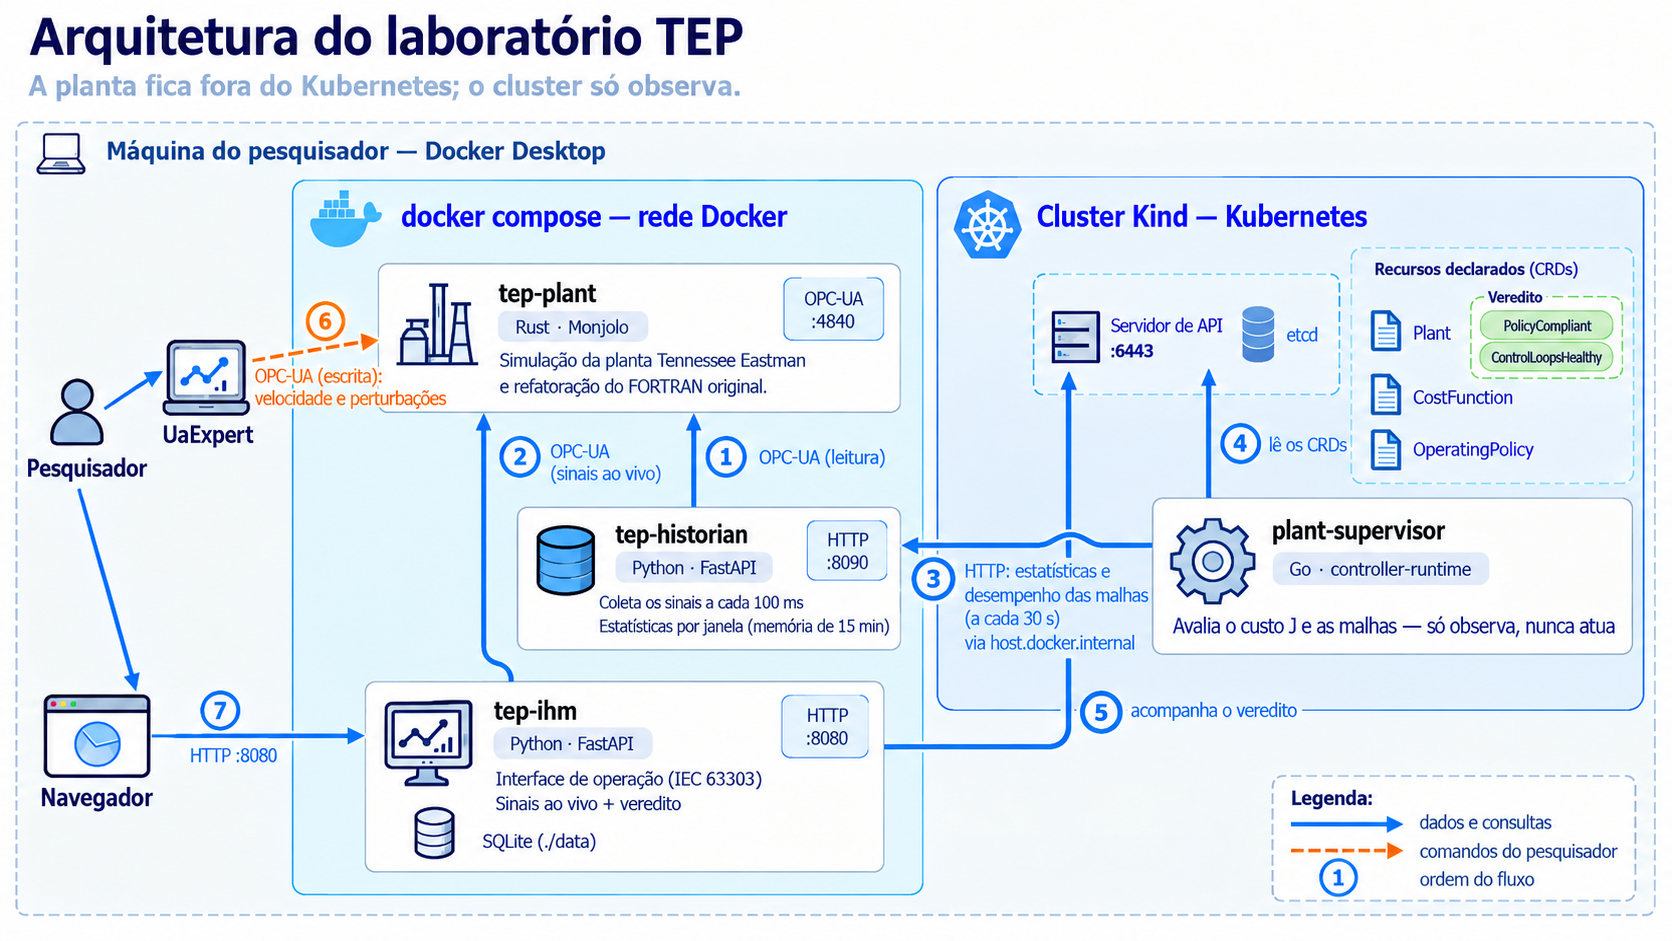
\includegraphics[width=\textwidth]{imagens/tep-arquitetura-laboratorio.png}
	\fonte{Elaborado pelo autor.}
	\label{fig:arq_lab}
\end{figure}

À direita fica o \textit{cluster} Kind.\footnote{O Kind (\textit{Kubernetes in Docker}) é uma ferramenta para rodar \textit{clusters} Kubernetes locais usando \textit{containers} Docker como nós (\url{https://kind.sigs.k8s.io/}).} Em vez de usar máquinas separadas, o Kind cria um \textit{container} Docker que faz o papel de um computador inteiro: dentro dele rodam o Kubernetes e o containerd — e sim, é uma espécie de Docker dentro de um Docker —, que é quem executa os \textit{containers} do \textit{cluster}. É ali que ficam os recursos que o usuário declara com o \texttt{kubectl}, como a política de operação, e o \texttt{plant-supervisor}, escrito em Go, que os avalia. A cada 30~s, ele pede ao \textit{historian} as estatísticas da janela de tempo e o desempenho das malhas (3), avalia a planta e grava o veredito (4), que a IHM acompanha (5). Os detalhes desse lado ficam para a Seção~\ref{sec:supervisor}. A planta fica fora do Kubernetes e, no escopo deste trabalho, o supervisor só observa: ele não escreve na planta. Fazer o supervisor agir sobre ela para que a política seja cumprida fica para trabalhos futuros, como já indicado no P5. Quem age sobre ela é o pesquisador, que pode mudar a velocidade da simulação e ligar distúrbios pelo OPC~UA, com um cliente de uso geral como o UaExpert (6), e acompanha tudo pela IHM no navegador (7).

\subsection{Componentes e fluxo de informação}
\label{subsec:componentes}

Antes de entrar no código, vale descrever o que cada componente faz quando tudo está rodando e conversando.

O código original do TEP, publicado em FORTRAN por \citeonline{DOWNS1993}, é procedural e roda em lote: um programa principal integra o modelo por um horizonte fixo, escreve os resultados e termina. O \texttt{tep-plant} reimplementa o modelo como um serviço que não para. Ele avança no tempo, em tempo real ou acelerado, e deixa que outros programas conversem com a simulação enquanto ela roda. Isso exige mais do ponto de vista de engenharia de software, porque a simulação e a comunicação precisam rodar em paralelo sem atrapalhar uma à outra; o Apêndice~\ref{apendice:monjolo} trata dessa parte.

Para um cliente OPC~UA, a planta simulada se parece com uma planta real: ele vê sinais que mudam com o tempo e pode escrever nos atuadores, sem precisar saber que do outro lado há uma simulação. O \texttt{tep-plant} é a fonte da informação, é ali que tudo começa, e por isso ele não consulta nenhum outro componente. Por dentro, ele resolve continuamente as equações diferenciais do modelo e publica os resultados, sem guardar nada: cada valor novo sobrescreve o anterior. É também dentro dele que ficam as malhas regulatórias, ou seja, é aqui que o P4 acontece.

O \texttt{tep-historian} é um dos clientes da planta. Ele coleta por OPC~UA todos os sinais que a planta publica e guarda os últimos 15 minutos de cada um, então já retém alguma informação. Sobre esses dados, calcula estatísticas por janela de tempo e o índice de desempenho das malhas, e oferece os resultados por uma API HTTP. Ou seja, o \textit{historian} é cliente da planta e, ao mesmo tempo, um serviço para quem precisa dessas análises.

A \texttt{tep-ihm} é o outro cliente. Com ela rodando, basta abrir o endereço dela no navegador para ver a tela da Figura~\ref{fig:ihm}, que é a única representação visual do que acontece dentro da planta. A IHM é uma aplicação web completa, com o servidor em Python e a interface em JavaScript, desenhada no navegador do usuário. Ela mostra as medições e as variáveis manipuladas, mas não tudo o que existe dentro da simulação.

\begin{figure}[htbp]
	\centering
	\caption{A IHM no navegador: o fluxograma do TEP com as medições (XMEAS) e as variáveis manipuladas (XMV) atualizadas ao vivo.}
	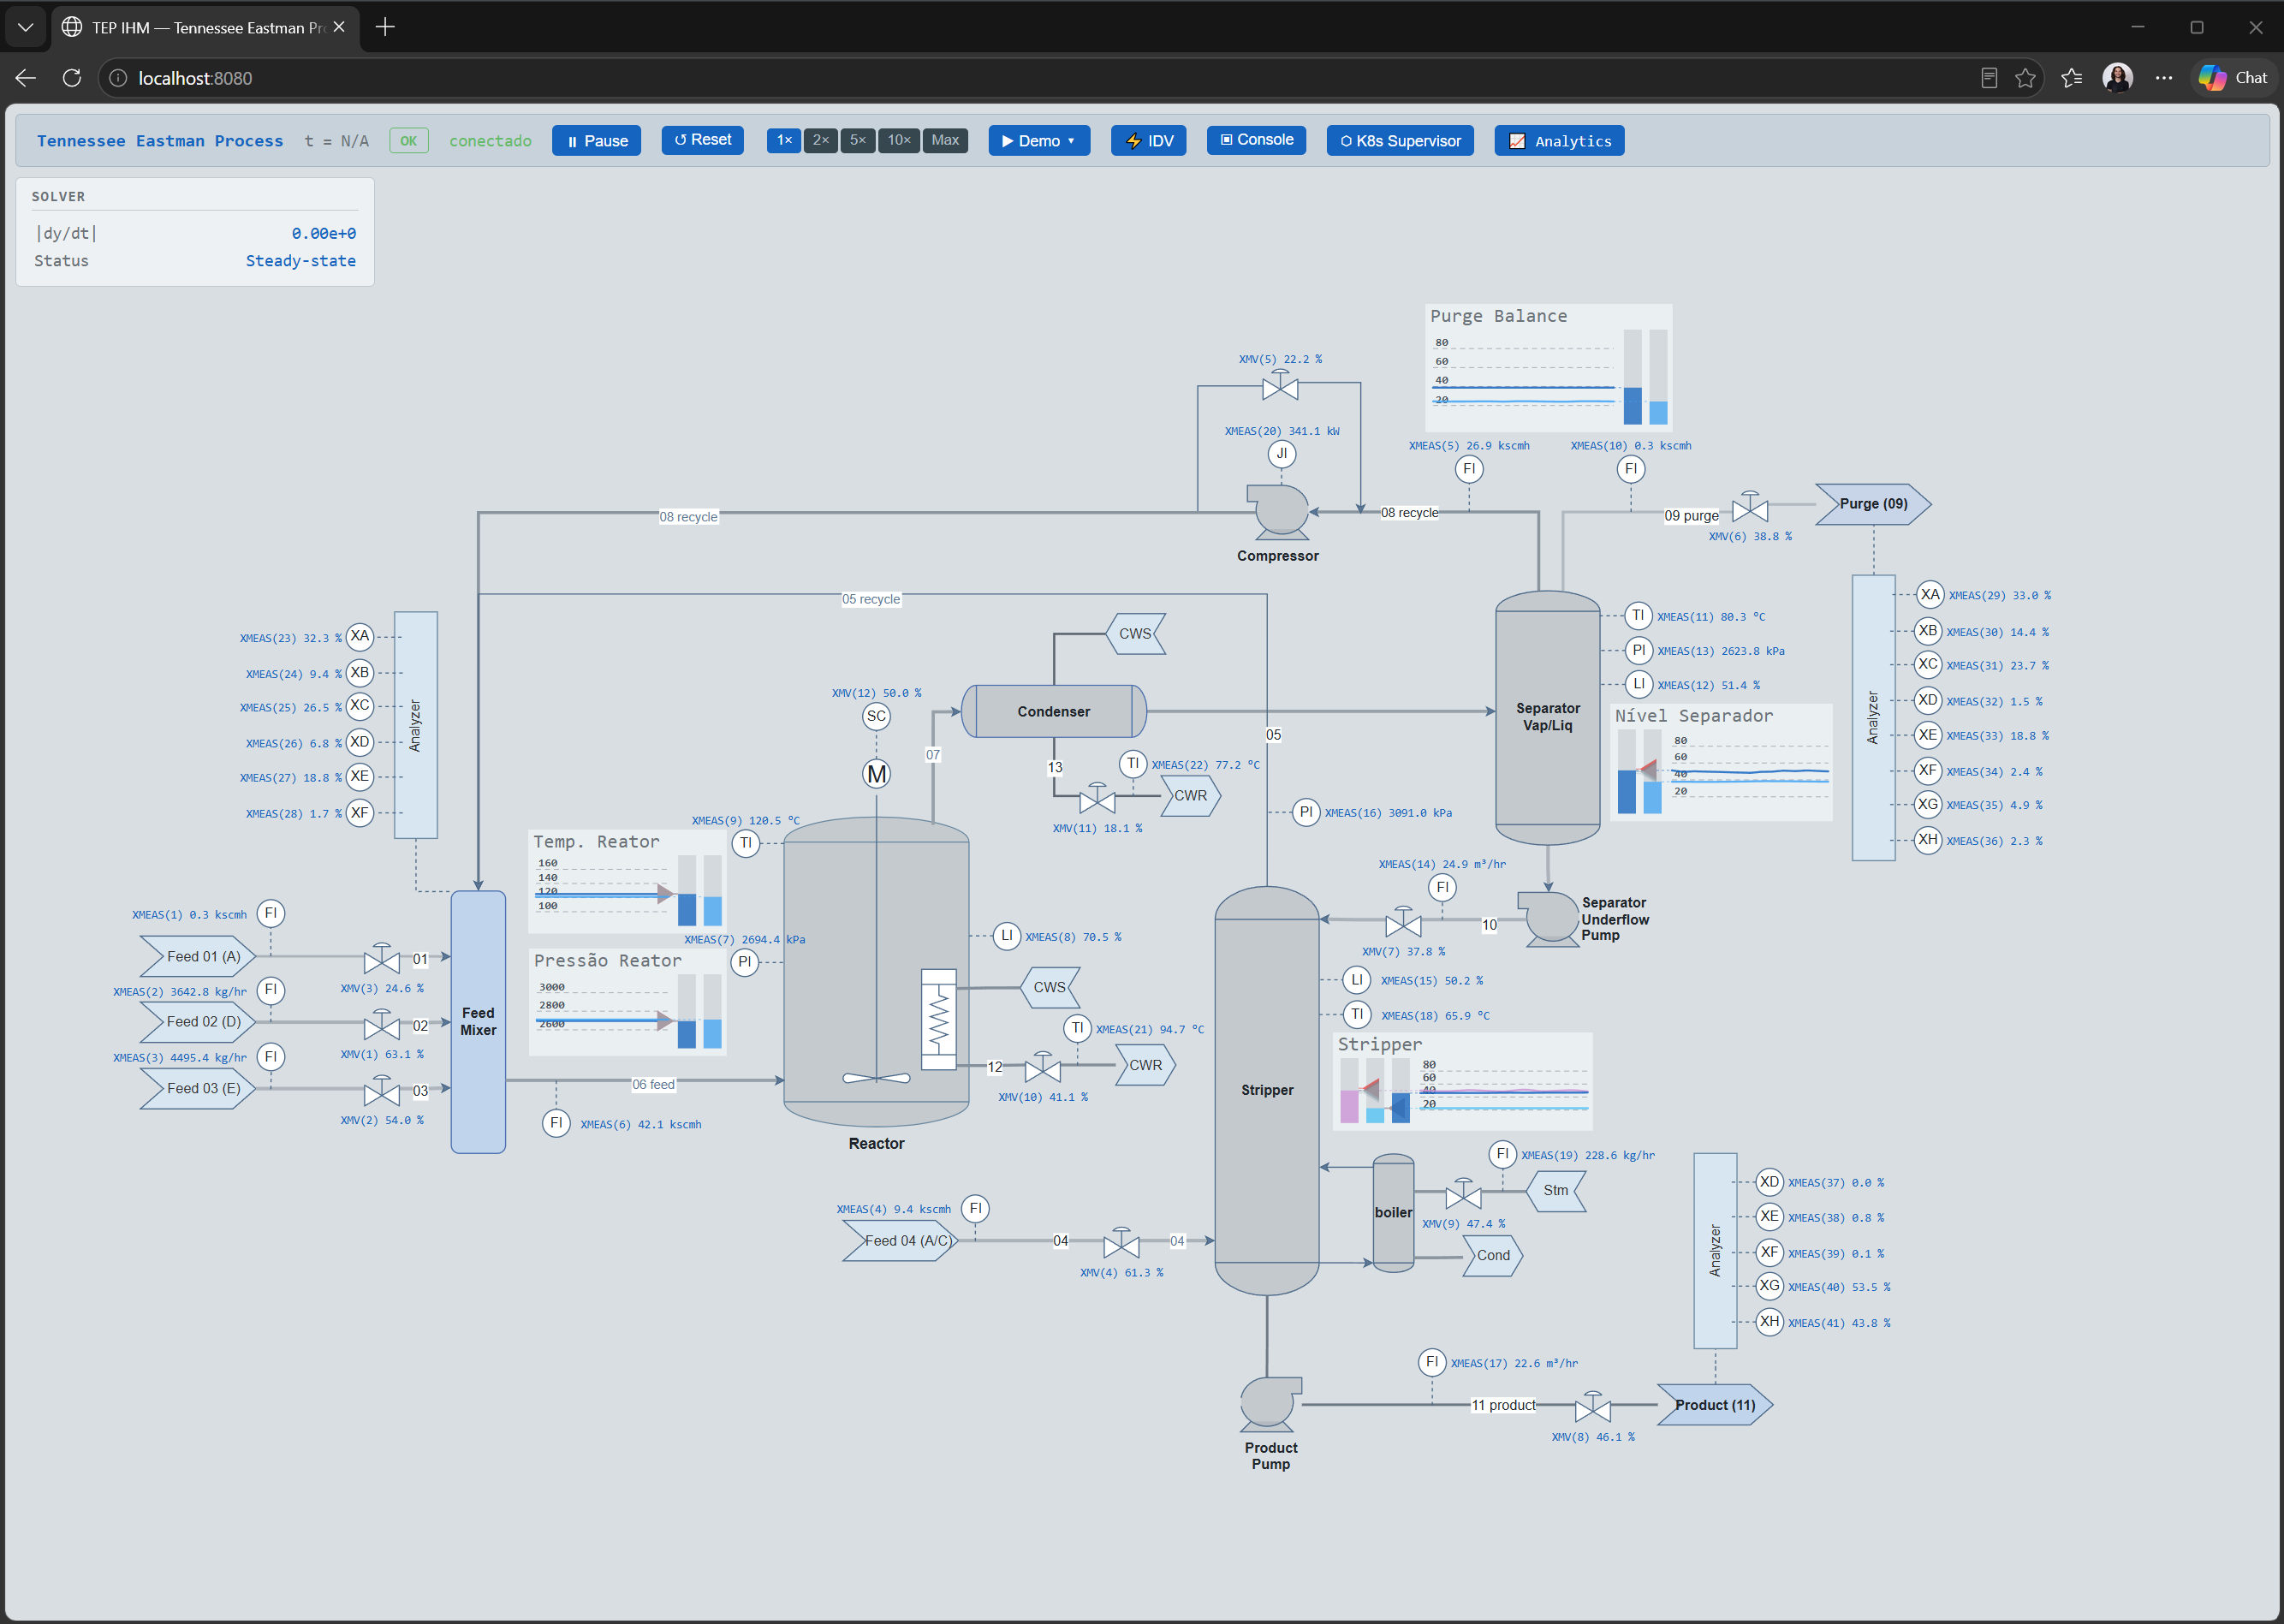
\includegraphics[width=\textwidth]{imagens/tep-ihm-no_navegador.png}
	\fonte{Elaborado pelo autor.}
	\label{fig:ihm}
\end{figure}

No começo, a IHM também enviava comandos para a planta, como sugerem os botões da barra superior da Figura~\ref{fig:ihm}. Com as refatorações sucessivas, essas funções deixaram de funcionar e ainda não foram corrigidas. Por isso, os comandos dados à planta neste trabalho foram todos enviados pelo UaExpert, um cliente OPC~UA de uso geral que dá acesso direto a todos os sinais. Ele faz, para o OPC~UA, o papel que o Postman faz para APIs HTTP: permite consultar sinais e enviar comandos sem escrever código.

Por fim, o \texttt{plant-supervisor} é um \textit{pod} no \textit{cluster} Kubernetes que consulta o \textit{historian} periodicamente. A API do \textit{historian} segue um contrato definido, e é por ele que o supervisor pede as estatísticas de que precisa. Do lado do supervisor fica a avaliação da política: o custo $J$, as metas, os limites e o julgamento das malhas. A própria função de custo do TEP não está no código do supervisor: ela é declarada num manifesto, como um recurso do Kubernetes, assunto da Seção~\ref{sec:supervisor}.


% -------------------------------------------------------------------------
\section{Planta simulada}
\label{sec:planta}

O \texttt{tep-plant} é a reescrita, em Rust, do modelo de \citeonline{DOWNS1993}. A referência é o código original em FORTRAN~77, na versão distribuída pelo grupo de Richard Braatz, da Universidade de Illinois.\footnote{\url{https://github.com/camaramm/tennessee-eastman-profBraatz}. Os números de linha citados nesta seção são os dos arquivos desse repositório.} Nesse código, o modelo da planta fica numa sub-rotina, a \texttt{TEFUNC}, que recebe o vetor de estados \texttt{YY} e devolve as derivadas \texttt{YP}. Os 50 estados são acessados pela posição no vetor: \texttt{YY(37)}, por exemplo, é a temperatura da água de resfriamento que sai do reator. As grandezas intermediárias, como a temperatura e a pressão do reator, ficam em blocos \texttt{COMMON}, que são variáveis globais compartilhadas entre as sub-rotinas.

No \texttt{tep-plant}, o código é dividido em pastas, uma para cada tipo de coisa que existe numa planta: \texttt{units/} para as cinco unidades de processo, \texttt{controllers/} para as malhas de controle, \texttt{sensors/} e \texttt{actuators/} para os instrumentos, \texttt{disturbance/} para os distúrbios, \texttt{physics/} para as constantes físico-químicas e \texttt{diagnostics/} para a detecção de parada de emergência, que depende de mais de uma unidade. Quem escreve esse código descreve o processo e o controle. A integração numérica, a ordem dos cálculos, as \textit{threads} e o servidor OPC~UA ficam no monjolo e não aparecem aqui. A intenção é que o usuário típico, um engenheiro químico, consiga ler e mudar a planta sem conhecer essa parte.

Os trechos de código desta seção usam alguns recursos do Rust e do monjolo que não são óbvios, como os atributos escritos entre \texttt{\#[} e \texttt{]} sobre as estruturas. Eles não são explicados aqui: cada um tem uma seção no Apêndice~\ref{apendice:monjolo}, indicada em nota de rodapé.

Esta seção descreve o \texttt{tep-plant} na versão 2.1.0-alpha, a mais recente do ramo principal. Os experimentos com o supervisor, no Capítulo~\ref{cha:resultados}, usaram também a versão 2.0.0, que só difere desta nas malhas de controle (Seção~\ref{subsec:malhas}).

\subsection{Unidades e seus cálculos}
\label{subsec:unidades}

As cinco unidades são o \texttt{Feed}, o \texttt{Reactor}, o \texttt{Separator}, o \texttt{Stripper} e o \texttt{Compressor}, cada uma num arquivo da pasta \texttt{units/}. Uma unidade guarda os seus estados integrados, que são o inventário de cada componente químico e a energia do vaso, e divide os seus cálculos em tarefas com nome. O reator, por exemplo, tem cinco tarefas:
\begin{itemize}
	\item \texttt{physical\_state}: a partir dos estados, calcula a temperatura, a pressão, os volumes de líquido e de vapor e as taxas das quatro reações;
	\item \texttt{flow\_to\_separator}: calcula a vazão da corrente 7, do reator para o separador;
	\item \texttt{heat\_exchange}: calcula o calor retirado pela água de resfriamento;
	\item \texttt{mass\_and\_energy\_balance}: monta as derivadas dos nove estados do reator;
	\item \texttt{xmeas\_readings}: converte a pressão, o nível e as temperaturas para as unidades das medições XMEAS.
\end{itemize}

As outras unidades seguem o mesmo padrão. O \texttt{Feed} calcula as vazões das quatro alimentações a partir da posição das válvulas, a composição da alimentação de A e C e a temperatura da alimentação de D. O \texttt{Separator}, o \texttt{Stripper} e o \texttt{Compressor} têm, além das tarefas equivalentes às do reator, a tarefa do analisador de composição que fica em cada um: o da purga no separador, o do produto no \textit{stripper} e o da alimentação do reator no compressor. Ao todo, são 32 tarefas. As quatro reações também são escritas pelo nome, como \texttt{A + C + D -> G}, e não por índices de vetor.\footnote{As misturas e as reações estão na Seção~\ref{apC:mistura}.}

O Código~\ref{cod:fortran_calor} mostra como o FORTRAN calcula o calor retirado do reator. \texttt{VLR} é o volume de líquido do reator, \texttt{AGSP} é a velocidade do agitador, e \texttt{TWR} e \texttt{TCR} são as temperaturas da água de resfriamento e do reator. Essas variáveis vêm dos blocos \texttt{COMMON} e foram calculadas em outros pontos da \texttt{TEFUNC}, que precisam ter rodado antes. Quem lê o trecho precisa saber de onde vem cada uma e manter a ordem das linhas.

\noindent\begin{minipage}{\linewidth}
\begin{lstlisting}[language={[77]Fortran}, caption={Calor retirado do reator no FORTRAN}, label={cod:fortran_calor}]
      IF(VLR/7.8.GT.50.0)THEN
      UARLEV=1.0
      ELSEIF(VLR/7.8.LT.10.0)THEN
      UARLEV=0.0
      ELSE
      UARLEV=0.025*VLR/7.8-0.25
      ENDIF
      UAR=UARLEV*(-0.5*AGSP**2
     .+2.75*AGSP-2.5)*855490.D-6
      QUR=UAR*(TWR-TCR)
     .*(1.D0-0.35D0*TESUB8(10,TIME))
\end{lstlisting}
\fonte{\citeonline{DOWNS1993}, arquivo \texttt{teprob.f}, linhas 663 a 673.}
\end{minipage}

O Código~\ref{cod:rust_calor} mostra a mesma conta no \texttt{tep-plant}. As entradas aparecem com o nome completo, depois de \texttt{need::}, e as saídas, depois de \texttt{offer::}. A tarefa não recebe parâmetros e não devolve nada: o próprio corpo diz o que ela lê e o que ela publica, e o monjolo usa essa informação para descobrir em que ordem rodar as tarefas de todas as unidades.\footnote{Os atributos \texttt{\#[...]} estão explicados na Seção~\ref{apC:atributos}; o \texttt{need::} e o \texttt{offer::}, nas Seções~\ref{apC:registro} e~\ref{apC:parametros}; e a ordem das tarefas, na Seção~\ref{apC:ordem}.} O \texttt{0.0} no fim da conta do calor é o lugar onde entraria o distúrbio IDV(17), que não foi implementado (Seção~\ref{subsec:disturbios}).

\noindent\begin{minipage}{\linewidth}
\begin{lstlisting}[language=Rust, caption={Calor retirado do reator no \texttt{tep-plant}}, label={cod:rust_calor}]
#[monjolo::dynamic_model(tasks)]
pub struct Reactor {
    /* ... inventários de vapor e de líquido */
    #[state]
    #[config(key = "state.reactor.energy")]
    #[offer(key = "reactor.state.enthalpy")]
    enthalpy: f64,
    constants: TepConstants,
}

#[monjolo::tasks(species = TEP_SPECIES, len = 8)]
impl Reactor {
    /* ... physical_state, flow_to_separator */
    #[task]
    fn heat_exchange(&self) {
        let agitation_factor = (need::agitator__speed + 150.0) / 100.0;
        let level = need::reactor__liquid_volume / 7.8;
        let uar_level = if level > 50.0 {
            1.0
        } else if level < 10.0 {
            0.0
        } else {
            0.025 * level - 0.25
        };
        let uar = uar_level
            * (-0.5 * agitation_factor * agitation_factor
                + 2.75 * agitation_factor - 2.5)
            * 855490e-6;
        let twr = REACTOR_COOLING_WATER_RETURN;

        offer::heat__reactor_heat =
            uar * (twr - need::reactor__temperature) * (1.0 - 0.35 * 0.0);
        offer::heat__reactor_cooling_water_return = twr;
    }
    /* ... mass_and_energy_balance, xmeas_readings */
}
\end{lstlisting}
\fonte{Elaborado pelo autor. \texttt{tep-plant}, arquivo \texttt{src/units/reactor.rs} (trecho).}
\end{minipage}

% *TODO* → achei isso confuso e mal explicado

Há uma diferença em relação ao FORTRAN, visível na linha 29 do \texttt{twr}. Nas versões do \texttt{tep-plant} usadas nos experimentos deste trabalho, a temperatura da água de resfriamento que sai do reator e a que sai do condensador do separador são constantes, iguais às do caso base. No FORTRAN, elas são estados integrados. A cópia do FORTRAN usada como referência durante boa parte do trabalho estava truncada e não tinha essas duas equações; uma fórmula aproximada deixou o reator instável, e as temperaturas foram fixadas. Com o arquivo original completo, a versão integrada foi refeita numa linha de trabalho paralela, que ainda não foi usada nos experimentos.

\subsection{Controladores}
\label{subsec:malhas}

A planta tem três malhas de controle, cada uma num arquivo da pasta \texttt{controllers/} (Figura~\ref{fig:tep_malhas}):
\begin{itemize}
	\item a pressão do reator (XMEAS 7), controlada pela válvula de purga (XMV 6);
	\item o nível do separador (XMEAS 12), controlado pela válvula de saída de fundo do separador (XMV 7);
	\item o nível do \textit{stripper} (XMEAS 15), controlado pela válvula de produto (XMV 8).
\end{itemize}

Na figura, os controladores têm os nomes que se usam em fluxogramas de processo: PIC é um controlador de pressão e LIC, um controlador de nível, seguidos do número da malha. As linhas tracejadas ligam a medição ao controlador e o controlador à válvula.

\begin{figure}[htbp]
	\centering
	\caption{Malhas de controle do \texttt{tep-plant} sobre o fluxograma do TEP.}
	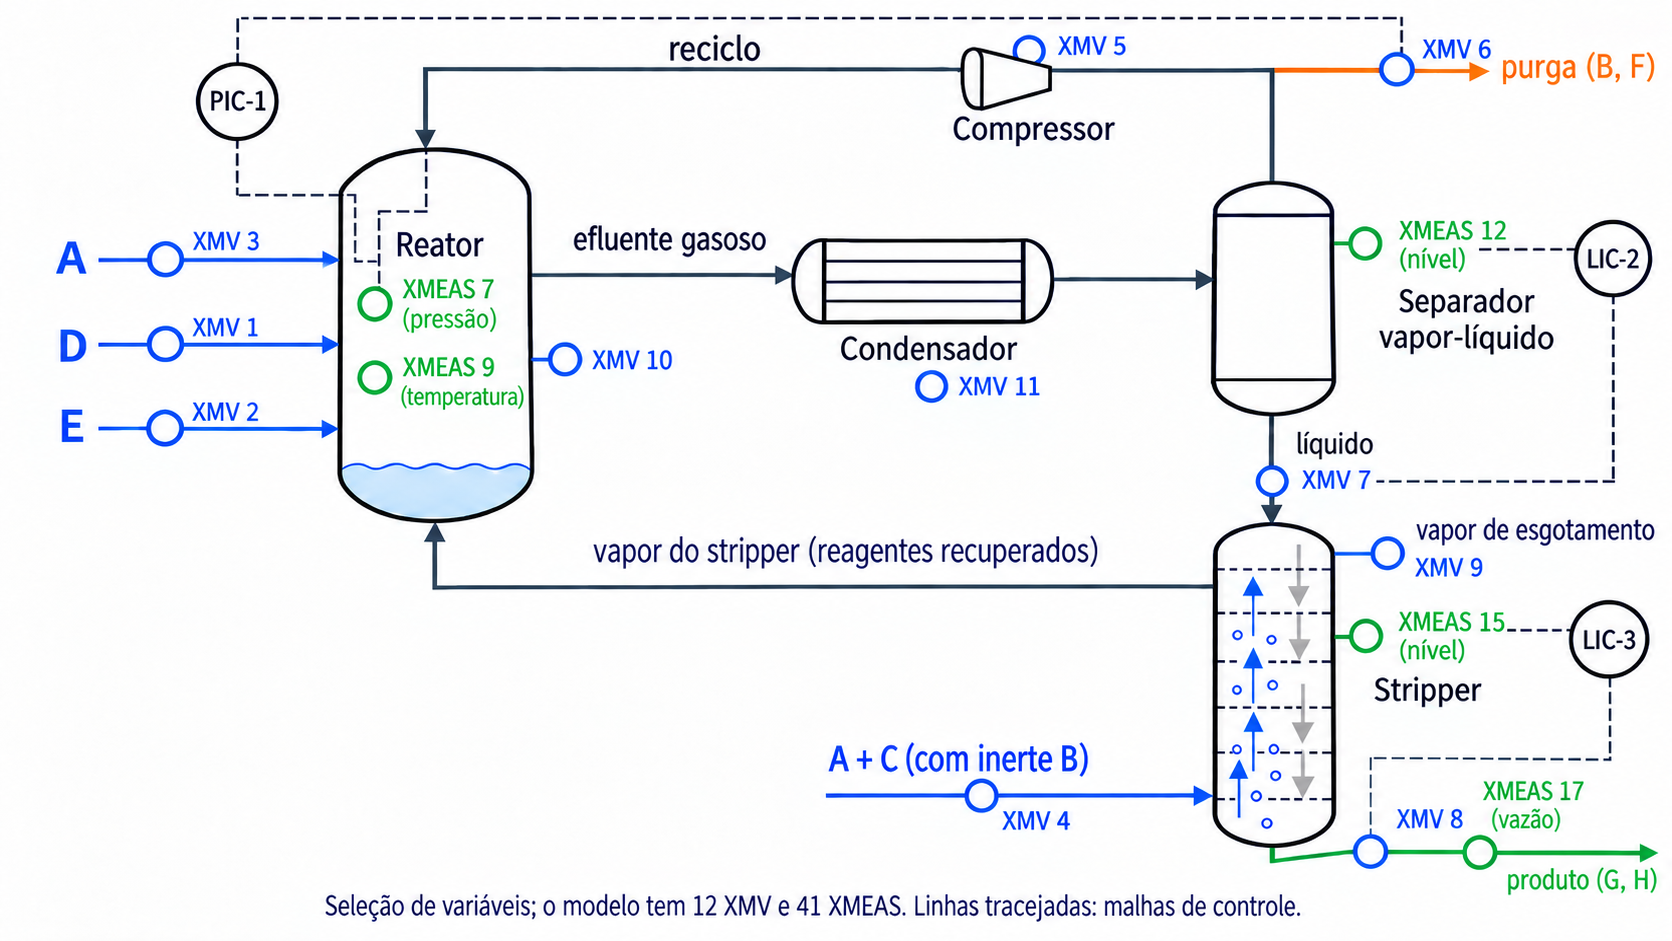
\includegraphics[width=0.95\textwidth]{imagens/tep-malhas-controle.png}
	\fonte{Elaborado pelo autor, com base em \citeonline{DOWNS1993}.}
	\label{fig:tep_malhas}
\end{figure}

Com ação só proporcional, essas três malhas mantiveram a planta operando no Modo~1 sem distúrbio, e uma quarta malha, do nível do reator para a alimentação de A, piorou a planta em vez de ajudar (Seção~\ref{sec:experimentos_planta}). Essa é a versão 2.0.0. Depois que, só com a ação proporcional, a planta não voltou ao ponto de operação após o distúrbio IDV(6), as malhas passaram a proporcionais-integrais (PI), na versão 2.1.0-alpha. Com PI e sem uma malha de nível do reator, porém, a planta deriva mesmo sem distúrbio e se perde em cerca de 33~h. Os dois experimentos são discutidos no Capítulo~\ref{cha:resultados}. Os ganhos são $K_c = 0{,}1$~\%/kPa e $\tau_i = 20$~min na malha de pressão, e $K_c = 1{,}0$~\%/\% e $\tau_i = 200$~min nas malhas de nível. Os \textit{setpoints} são 2705~kPa e 50~\%. Na versão 2.0.0, os ganhos e os \textit{setpoints} são os mesmos, sem o termo integral.

O Código~\ref{cod:rust_pi} mostra a malha de pressão. Os campos marcados com \texttt{\#[sensor]} e \texttt{\#[actuator]} dizem, pelo nome, qual medição a malha lê e qual válvula ela comanda. O campo marcado com \texttt{\#[state]} é a integral do erro: ela é um estado, integrado junto com a planta, e a função \texttt{control} devolve a sua derivada. Quando a válvula satura no sentido do erro, a derivada volta zero, para a integral não crescer à toa (\textit{anti-windup}).\footnote{O motivo de a integral não ser somada dentro de \texttt{control} está na Seção~\ref{apC:integracao}.}

\noindent\begin{minipage}{\linewidth}
\begin{lstlisting}[language=Rust, caption={Malha PI da pressão do reator no \texttt{tep-plant}}, label={cod:rust_pi}]
#[monjolo::controller(name = "reactor_pressure_control")]
pub struct ReactorPressureControl {
    #[sensor(key = "xmeas.reactor.pressure")]
    pressure: f64,
    #[actuator(key = "valve.purge.position")]
    purge: f64,
    #[state(key = "controller.reactor_pressure.integral")]
    integral: f64,
}

impl ReactorPressureControl {
    fn control(&self) -> f64 {
        const KC: f64 = 0.1;
        const TI_HOURS: f64 = 20.0 / 60.0;
        const SETPOINT: f64 = 2705.0;
        const BIAS: f64 = 40.06;

        let error = self.pressure().read() - SETPOINT;
        let raw = BIAS + KC * (error + self.integral() / TI_HOURS);
        self.purge().write(raw.clamp(0.0, 100.0));

        let winding_up = (raw > 100.0 && KC * error > 0.0)
            || (raw < 0.0 && KC * error < 0.0);
        if winding_up { 0.0 } else { error }
    }
}
\end{lstlisting}
\fonte{Elaborado pelo autor. \texttt{tep-plant}, arquivo \texttt{src/controllers/reactor\_pressure\_control.rs}, sem os comentários.}
\end{minipage}

O programa de demonstração do FORTRAN também traz um controlador PI, para o nível do \textit{stripper} (Código~\ref{cod:fortran_pi}). Os dois têm tamanho parecido. A diferença está em como cada um chega aos dados: o FORTRAN lê \texttt{XMEAS(15)} e escreve \texttt{XMV(8)} pela posição, por meio de blocos \texttt{COMMON}, e guarda o erro anterior, \texttt{ERROLD}, numa variável global entre uma chamada e outra.

\noindent\begin{minipage}{\linewidth}
\begin{lstlisting}[language={[77]Fortran}, deletekeywords={ERR}, caption={Controlador PI do programa de demonstração do FORTRAN}, label={cod:fortran_pi}]
      SUBROUTINE CONTRL
      DOUBLE PRECISION XMEAS, XMV
      COMMON /PV/ XMEAS(41), XMV(12)
      DOUBLE PRECISION SETPT, GAIN, TAUI, ERROLD, DELTAT
      COMMON /CTRL/ SETPT, GAIN, TAUI, ERROLD, DELTAT
      DOUBLE PRECISION ERR, DXMV
      ERR = SETPT - XMEAS(15)
      DXMV = GAIN * ( (ERR - ERROLD) + ERR * DELTAT * 60.0 / TAUI )
      XMV(8) = XMV(8) - DXMV
      ERROLD = ERR
      RETURN
      END
\end{lstlisting}
\fonte{\citeonline{DOWNS1993}, arquivo \texttt{temain.f}, sub-rotina \texttt{CONTRL}, sem os comentários.}
\end{minipage}

\subsection{Sensores e atuadores}
\label{subsec:sensores_atuadores}

Os sensores e os atuadores são as peças mais simples da planta (Código~\ref{cod:rust_instrumentos}). Um sensor é declarado em duas linhas, com o nome da medição que ele expõe e o desvio padrão do ruído gaussiano, o mesmo da tabela \texttt{XNS} do FORTRAN: 0,3~kPa para a pressão do reator. A conversão para a unidade da medição é feita pela própria unidade de processo, na tarefa \texttt{xmeas\_readings}. São 42 sensores: as 41 medições XMEAS e um sinal que indica a parada de emergência. Uma diferença em relação ao FORTRAN é que os analisadores de composição (XMEAS 23 a 41) aqui são contínuos. No FORTRAN, eles fazem uma amostra a cada 0,1~h ou 0,25~h e seguram o valor até a amostra seguinte.

Os 12 atuadores (XMV 1 a 12) seguem a mesma ideia. Cada um tem o comando recebido e a posição real da válvula, que é um estado e segue o comando com um atraso de primeira ordem, $\mathrm{d}x/\mathrm{d}t = (u - x)/\tau$. As constantes de tempo são as da tabela \texttt{VTAU} do FORTRAN: 5~s para a válvula de água de resfriamento do reator, por exemplo. A posição inicial vem do arquivo de configuração, na chave indicada em \texttt{config}.

Cada sensor e cada atuador declarado vira, sem nenhuma linha a mais, um nó com o mesmo nome na pasta \texttt{Signals} do servidor OPC~UA. É isso que o \textit{historian}, a IHM e o UaExpert enxergam.\footnote{Como os componentes se registram sozinhos está na Seção~\ref{apC:registro_auto}; como o adaptador OPC~UA monta os nós, na Seção~\ref{apC:opcua}.}

\noindent\begin{minipage}{\linewidth}
\begin{lstlisting}[language=Rust, caption={Um sensor e um atuador no \texttt{tep-plant}}, label={cod:rust_instrumentos}]
#[monjolo::sensor(key = "xmeas.reactor.pressure", noise = 0.3)]
pub struct ReactorPressure;

#[monjolo::actuator(key = "valve.reactor_cooling_water.position",
                    config = "state.valves.reactor_cooling_water")]
pub struct ReactorCoolingWater {
    #[command]
    command: f64,
    #[state]
    position: f64,
}

impl ReactorCoolingWater {
    fn dynamics(&self) -> f64 {
        let tau = 5.0 / 3600.0;
        (self.command() - self.position()) / tau
    }
}
\end{lstlisting}
\fonte{Elaborado pelo autor. \texttt{tep-plant}, arquivos \texttt{src/sensors/reactor\_pressure.rs} e \texttt{src/actuators/reactor\_cooling\_water.rs}, sem os comentários.}
\end{minipage}

A Figura~\ref{fig:uaexpert} mostra o que um cliente OPC~UA enxerga. No UaExpert conectado à planta, a pasta \texttt{Signals} fica dentro de \texttt{Objects}, e cada nó tem o nome da chave declarada no código: \texttt{xmeas.reactor.pressure} é a pressão do reator, \texttt{valve.purge.position} é a posição da válvula de purga, e assim por diante. Na mesma pasta ficam o nó \texttt{clock.t\_h}, com o tempo simulado em horas, o sinal de parada de emergência e um nó para cada distúrbio implementado, com valor 0 quando desligado (Seção~\ref{subsec:disturbios}). Os nós dos atuadores e dos distúrbios aceitam escrita. Por eles e pelos métodos de controle da simulação, como o de velocidade, foram dados os comandos deste trabalho.

\begin{figure}[htbp]
	\centering
	\caption{O UaExpert conectado à planta: a pasta \texttt{Signals} no espaço de endereçamento e os valores dos seus nós.}
	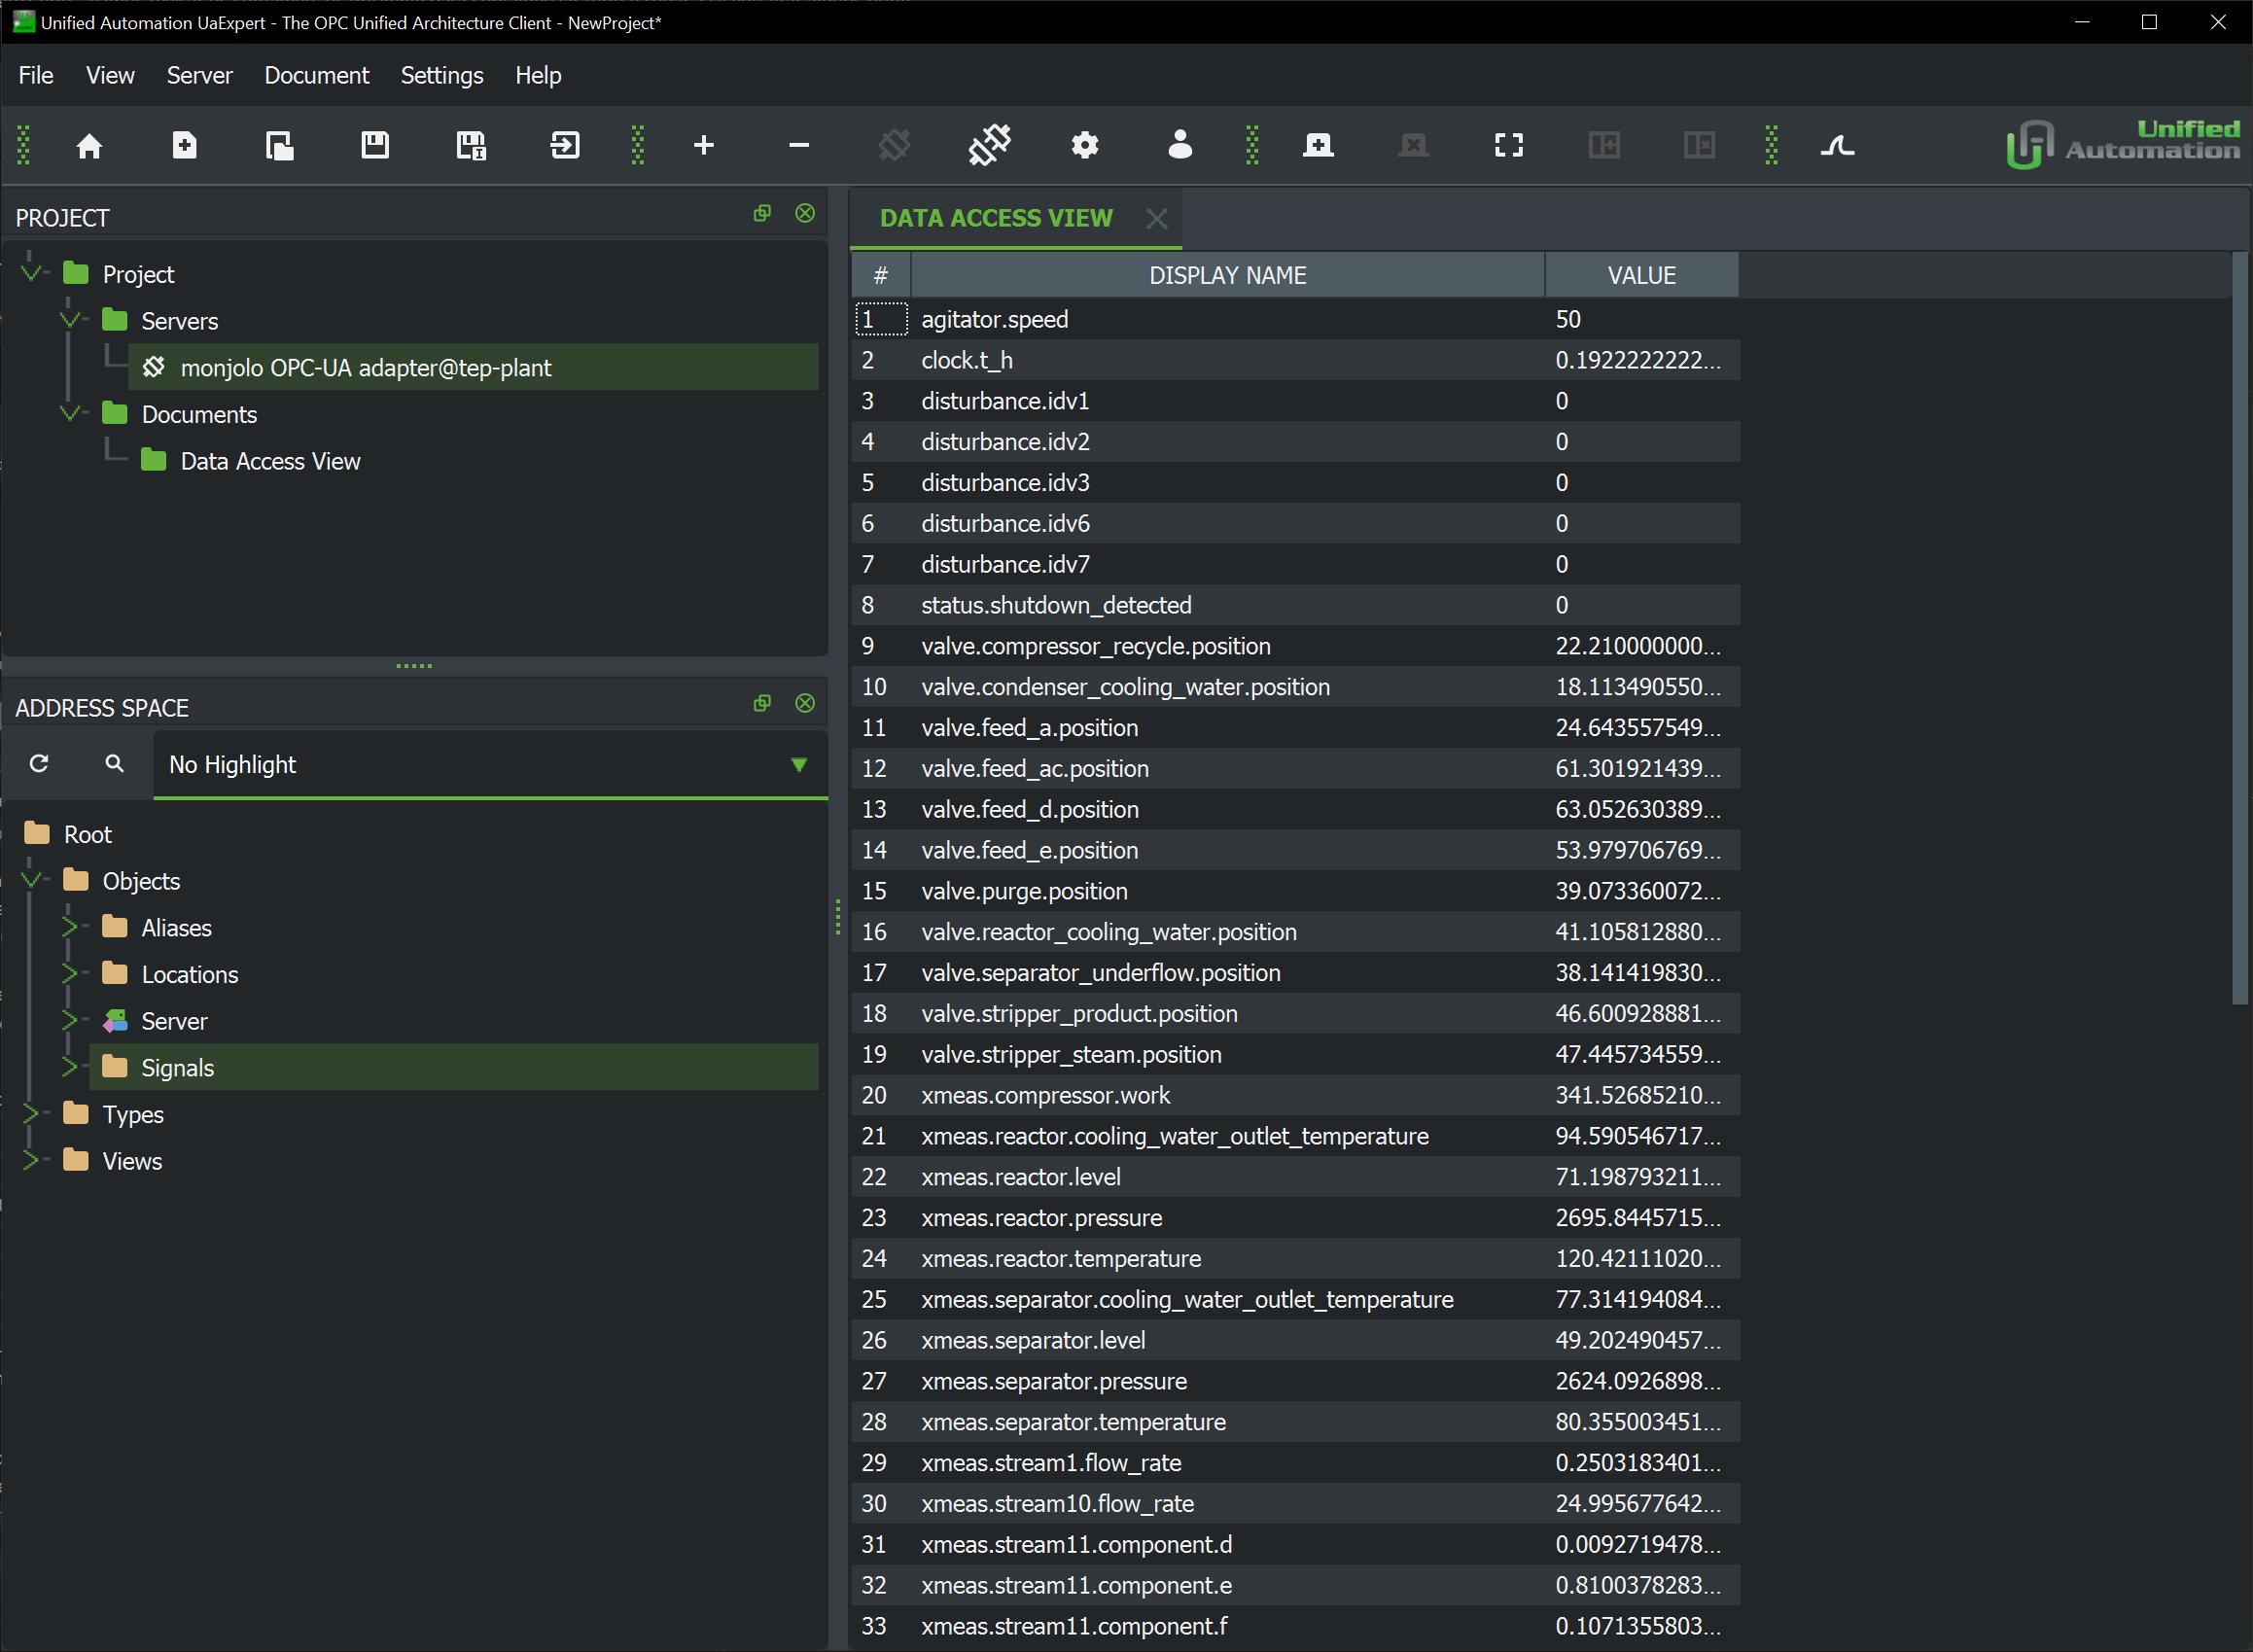
\includegraphics[width=\textwidth]{imagens/UaExpert-conectado em tep-plant.png}
	\fonte{Elaborado pelo autor.}
	\label{fig:uaexpert}
\end{figure}

\subsection{Distúrbios}
\label{subsec:disturbios}

\citeonline{DOWNS1993} definem 20 distúrbios, de IDV(1) a IDV(20). A regra seguida no \texttt{tep-plant} foi implementar cada distúrbio do jeito que o \texttt{teprob.f} implementa e não inventar nada onde o FORTRAN não define. Dos 20, cinco estão implementados (Tabela~\ref{tab:idvs}).

\begin{table}[htbp]
	\centering
	\caption{Situação dos distúrbios de Downs e Vogel no \texttt{tep-plant}.}
	\label{tab:idvs}
	\footnotesize
	\begin{tabular}{|c|>{\raggedright\arraybackslash}p{0.42\textwidth}|>{\raggedright\arraybackslash}p{0.36\textwidth}|}
		\hline
		\textbf{IDV} & \textbf{O que muda} & \textbf{Situação} \\
		\hline
		1, 2 & composição da alimentação 4 (razão A/C; teor de B), em degrau & implementados \\
		3 & temperatura da alimentação de D, em degrau & implementado \\
		6 & perda da alimentação de A, em degrau & implementado \\
		7 & pressão do cabeçalho de C, em degrau & implementado \\
		\hline
		4, 5 & temperatura de entrada da água de resfriamento, em degrau & sem efeito: a temperatura de saída da água é constante nesta versão \\
		8 a 13 & composições, temperaturas e cinética, aleatórios ou em deriva lenta & falta um gerador de sinal aleatório \\
		14, 15, 19 & válvulas travadas: as de água de resfriamento (14, 15) e as XMV 5, 7, 8 e 9 (19, desconhecido no artigo) & falta o mecanismo no atuador \\
		16 a 18, 20 & desconhecidos no artigo; aleatórios no \texttt{teprob.f} & falta um gerador de sinal aleatório \\
		\hline
	\end{tabular}
	\fonte{Elaborado pelo autor, com base em \citeonline{DOWNS1993} e no arquivo \texttt{teprob.f}.}
\end{table}

Os distúrbios aleatórios do FORTRAN usam um gerador próprio, que sorteia polinômios cúbicos em trechos (sub-rotinas \texttt{TESUB5}, \texttt{TESUB7} e \texttt{TESUB8}). No \texttt{tep-plant}, o mecanismo de distúrbios ainda só aceita uma transformação fixa do valor, sem estado que avance no tempo, e por isso cobre só os degraus. Os IDV(11), (12), (14) e (15) também agem sobre a água de resfriamento e, nesta versão, não teriam efeito mesmo se fossem implementados.

O Código~\ref{cod:rust_idv1} mostra o IDV(1). O distúrbio é um tipo próprio, num arquivo próprio, que intercepta a composição da alimentação 4 quando ela é publicada pelo \texttt{Feed}, tira 0,03 da fração de A e compensa em C. Nem o \texttt{Feed} nem o \texttt{Stripper}, que consome essa composição, sabem que o distúrbio existe.\footnote{O mecanismo de interceptação está na Seção~\ref{apC:disturbios}.} No FORTRAN, o mesmo distúrbio é um termo dentro da linha que calcula essa composição:
\begin{center}
	\texttt{XST(1,4)=TESUB8(1,TIME)-IDV(1)*0.03D0-IDV(2)*2.43719D-3}
\end{center}
Em linhas, o FORTRAN é mais curto; em troca, o cálculo da alimentação precisa conhecer todos os distúrbios que mexem nela. Os distúrbios são ligados e desligados pelo OPC~UA, escrevendo 1 ou 0 no nó com o nome do distúrbio, como \texttt{disturbance.idv1} (Figura~\ref{fig:uaexpert}).

\noindent\begin{minipage}{\linewidth}
\begin{lstlisting}[language=Rust, caption={O distúrbio IDV(1) no \texttt{tep-plant}}, label={cod:rust_idv1}]
#[monjolo::disturbance(
    key = "disturbance.idv1",
    intercepts = "flows.stream4_composition",
    components = ["a", "b", "c", "d", "e", "f", "g", "h"],
    species = TEP_SPECIES
)]
pub struct Idv1;

impl Idv1 {
    fn disturb(&self) -> Mixture<8> {
        let mut composition = self.raw().as_array();
        composition[0] -= 0.03;
        composition[2] = 1.0 - composition[0] - composition[1];
        Mixture::new(composition, &TEP_SPECIES)
    }
}
\end{lstlisting}
\fonte{Elaborado pelo autor. \texttt{tep-plant}, arquivo \texttt{src/disturbance/idv1.rs}, sem os comentários e as importações.}
\end{minipage}

\subsection{A função \texttt{main}}
\label{subsec:main}

O programa principal de demonstração do FORTRAN, no arquivo \texttt{temain.f}, mostra como o código foi pensado para ser usado (Código~\ref{cod:fortran_main}). Ele declara os mesmos blocos \texttt{COMMON}, chama \texttt{TEINIT} para iniciar os estados, ajusta o controlador e entra num laço de 1000 passos de 1~s. A cada passo, chama o controlador, imprime três variáveis e integra as derivadas pelo método de Euler. Depois dos 1000 passos, o programa termina. Para ligar um distúrbio, mudar a duração ou trocar o integrador, é preciso editar o arquivo e compilar de novo.

\noindent\begin{minipage}{\linewidth}
\begin{lstlisting}[language={[77]Fortran}, caption={Programa principal de demonstração do FORTRAN}, label={cod:fortran_main}]
      DOUBLE PRECISION XMEAS, XMV
      COMMON /PV/ XMEAS(41), XMV(12)
      INTEGER IDV
      COMMON /DVEC/ IDV(20)
      DOUBLE PRECISION SETPT, GAIN, TAUI, ERROLD, DELTAT
      COMMON /CTRL/ SETPT, GAIN, TAUI, ERROLD, DELTAT
      INTEGER I, NN, NPTS
      DOUBLE PRECISION TIME, YY(50), YP(50)
      NN = 50
      NPTS = 1000
      DELTAT = 1.0 / 3600.0
      CALL TEINIT(NN, TIME, YY, YP)
      SETPT  = XMEAS(15) + 15.0
      GAIN   = 2.0
      TAUI   = 5.0
      ERROLD = 0.0
      XMV(10) = 38.0
      DO 100 I = 1, 20
         IDV(I) = 0
 100  CONTINUE
      DO 1000 I = 1, NPTS
         CALL CONTRL
         CALL OUTPUT
         CALL INTGTR(NN, TIME, DELTAT, YY, YP)
 1000 CONTINUE
      STOP
      END
\end{lstlisting}
\fonte{\citeonline{DOWNS1993}, arquivo \texttt{temain.f}, programa principal, sem os comentários.}
\end{minipage}

No \texttt{tep-plant}, a função \texttt{main} tem uma instrução só (Código~\ref{cod:rust_main}). O \texttt{Runtime::bootstrap} lê o arquivo \texttt{application.toml}, que fica na raiz do projeto e guarda o estado inicial da planta e, se for preciso, a configuração do monjolo, como o método de integração e o endereço do servidor OPC~UA. Depois, descobre sozinho as unidades, os sensores, os atuadores, os controladores e os distúrbios declarados nas pastas e coloca a planta para rodar. O \texttt{run} mantém o programa vivo até alguém pedir para ele parar. A planta avança 1~s simulado a cada passo, integrada pelo método de Runge-Kutta de quarta ordem, e a velocidade, a pausa e o reinício são comandados pelo OPC~UA, com o programa rodando.\footnote{A linha \texttt{extern crate} e a descoberta automática dos componentes estão na Seção~\ref{apC:registro_auto}; o \texttt{bootstrap}, na Seção~\ref{apC:bootstrap}.}

\noindent\begin{minipage}{\linewidth}
\begin{lstlisting}[language=Rust, caption={A função \texttt{main} do \texttt{tep-plant}}, label={cod:rust_main}]
extern crate tennessee_eastman_process;

fn main() {
    monjolo::runtime::Runtime::bootstrap()
        .expect("Runtime::bootstrap encerrou com erro")
        .run();
}
\end{lstlisting}
\fonte{Elaborado pelo autor. \texttt{tep-plant}, arquivo \texttt{src/main.rs}, sem os comentários.}
\end{minipage}

\subsection{O que muda para quem escreve a planta}
\label{subsec:comparacao_fortran}

A Tabela~\ref{tab:linhas} compara o tamanho das duas implementações, contando só as linhas de código, sem comentários e sem linhas em branco. A comparação não é exata, porque as duas não fazem as mesmas coisas, mas mostra onde estão as diferenças.

\begin{table}[htbp]
	\centering
	\caption{Linhas de código no FORTRAN original e no \texttt{tep-plant}.}
	\label{tab:linhas}
	\footnotesize
	\begin{tabular}{|>{\raggedright\arraybackslash}p{0.40\textwidth}|>{\raggedright\arraybackslash}p{0.24\textwidth}|>{\raggedright\arraybackslash}p{0.24\textwidth}|}
		\hline
		\textbf{Parte} & \textbf{FORTRAN} & \textbf{\texttt{tep-plant}} \\
		\hline
		Programa principal & 27 (\texttt{temain.f}) & 6 (\texttt{main.rs}) \\
		Declarações no início da \texttt{TEFUNC} (blocos \texttt{COMMON} e variáveis) & 130 & nenhuma \\
		Cálculos da planta & 474 (resto da \texttt{TEFUNC}) & 528 (\texttt{units/}, 5 arquivos) \\
		Estado inicial e constantes & 474 (\texttt{TEINIT}) & 33 (\texttt{constants.rs}), mais os dados do \texttt{application.toml} \\
		Termodinâmica, ruído e geradores aleatórios & 214 (\texttt{TESUB1} a \texttt{TESUB8}) & no monjolo \\
		Um controlador PI & 12 (\texttt{CONTRL}) & 22 \\
		12 atuadores & 8 (um laço na \texttt{TEFUNC}) & 156 (12 arquivos de 13 linhas) \\
		42 sensores & dentro da \texttt{TEFUNC} & 84 (42 arquivos de 2 linhas) \\
		IDV(1) & um termo numa linha da \texttt{TEFUNC} & 17 (arquivo próprio) \\
		\hline
	\end{tabular}
	\fonte{Elaborado pelo autor, a partir dos arquivos \texttt{teprob.f} e \texttt{temain.f} de \citeonline{DOWNS1993} e da versão 2.1.0-alpha do \texttt{tep-plant}.}
\end{table}

O ganho não está no total de linhas, que é da mesma ordem nos dois casos: cerca de 1350 no FORTRAN e 1100 no \texttt{tep-plant}, que ainda não tem os distúrbios aleatórios e deixa para o monjolo a integração, o ruído e a rede. Em alguns pontos, o FORTRAN é até mais curto: as 12 válvulas cabem num laço de oito linhas, contra um arquivo de 13 linhas para cada atuador. A diferença está no que quem escreve a planta deixa de tratar. No \texttt{tep-plant} não há vetor de estados acessado por posição nem variáveis globais, e a ordem dos cálculos não depende da ordem das linhas. O programa principal deixou de ser um laço escrito à mão, e cada unidade, malha, instrumento ou distúrbio fica num arquivo próprio, com nome. Para acrescentar um sensor, bastam um arquivo de duas linhas e a linha que declara esse arquivo como módulo, e ele já aparece no OPC~UA. Os números por parte da Tabela~\ref{tab:linhas} não incluem os arquivos \texttt{mod.rs} e \texttt{lib.rs}, que só declaram os módulos e somam 148 linhas; o total de 1100 inclui.

% -------------------------------------------------------------------------
\section{\textit{Historian}}
\label{sec:historian}

O \texttt{tep-historian} é um programa em Python que fica entre a planta e o supervisor. Ele lê os sinais da planta por OPC~UA, guarda uma janela recente de cada um e responde, por HTTP, com estatísticas dessas janelas. Ele não sabe nada sobre o TEP: qualquer nó que aparecer na pasta \texttt{Signals} do servidor vira uma série, com o nome do nó. O que é da planta, como os sinais que entram na função de custo, fica só nos manifestos do Kubernetes (Seção~\ref{subsec:recursos}).

As dependências são poucas: a biblioteca \texttt{asyncua},\footnote{\url{https://github.com/FreeOpcUa/opcua-asyncio}.} para o cliente OPC~UA; o FastAPI,\footnote{\url{https://fastapi.tiangolo.com}.} com o servidor uvicorn, para a API HTTP; o pydantic, que vem com o FastAPI, para validar as requisições; e o NumPy, para o ajuste por mínimos quadrados. As dependências são gerenciadas com o Poetry, e a imagem Docker parte da imagem oficial \texttt{python:3.12-slim}. O programa é configurado por variáveis de ambiente: no laboratório, ele lê a planta a cada 100~ms e guarda 900~s (15 minutos) de cada sinal.

\subsection{Coleta dos sinais por OPC~UA}
\label{subsec:coleta}

A coleta roda numa tarefa assíncrona, iniciada junto com o servidor HTTP (Código~\ref{cod:coletor}). Ao conectar, o coletor procura a pasta \texttt{Signals} dentro de \texttt{Objects} e monta um dicionário com o nome de cada nó. A busca é pelo nome, e não por um identificador fixo, porque o servidor atribui os índices de \textit{namespace} quando sobe. Depois, a cada intervalo, o coletor lê todos os nós numa única chamada e grava os valores, todos com o mesmo instante. Valores booleanos, como o sinal de parada de emergência, viram 0 ou 1. Se a conexão cair, o coletor espera 3~s e tenta de novo, sem limite de tentativas: quando a planta volta, a coleta volta sozinha.

\noindent\begin{minipage}{\linewidth}
\begin{lstlisting}[language=Python, caption={Laço de coleta do \textit{historian}}, label={cod:coletor}]
async def run_collector(endpoint, buffer, state, interval_s, reconnect_s=3.0):
    from asyncua import Client

    while True:
        try:
            async with Client(url=endpoint) as client:
                nodes_by_name = await resolve_signal_nodes(client)
                names = list(nodes_by_name)
                nodes = [nodes_by_name[n] for n in names]
                state.connected = True
                while True:
                    raw = await client.read_values(nodes)
                    now = time.monotonic()
                    buffer.append(now, to_numeric(dict(zip(names, raw))))
                    await asyncio.sleep(interval_s)
        except Exception as e:
            state.connected = False
            state.last_error = f"{type(e).__name__}: {e}"
            await asyncio.sleep(reconnect_s)
\end{lstlisting}
\fonte{Elaborado pelo autor. \texttt{tep-historian}, arquivo \texttt{collector.py} (trecho simplificado).}
\end{minipage}

\subsection{Séries temporais em memória}
\label{subsec:series}

As séries ficam num objeto \texttt{SignalBuffer}, que guarda, para cada chave, uma fila de pares (instante, valor). Os instantes vêm de um relógio monotônico, que só anda para frente. A cada gravação, o que ficou mais velho que a retenção é descartado do início da fila (Código~\ref{cod:buffer}). Como o coletor grava todas as chaves no mesmo instante, as séries de chaves diferentes compartilham os instantes, o que facilita alinhar a variável medida com a saída do controlador no índice das malhas.

\noindent\begin{minipage}{\linewidth}
\begin{lstlisting}[language=Python, caption={Gravação e descarte no \textit{buffer} do \textit{historian}}, label={cod:buffer}]
def append(self, ts, values):
    for key, value in values.items():
        series = self._series.setdefault(key, deque())
        series.append((ts, float(value)))
    self._prune(ts)

def _prune(self, now):
    cutoff = now - self.retention_s
    for series in self._series.values():
        while series and series[0][0] <= cutoff:
            series.popleft()
\end{lstlisting}
\fonte{Elaborado pelo autor. \texttt{tep-historian}, arquivo \texttt{buffer.py} (trecho).}
\end{minipage}

Essa escolha tem dois limites. Primeiro, tudo fica só em memória: se o \textit{historian} reiniciar, o histórico some. Segundo, a janela é medida em tempo de relógio, e não em tempo simulado. Com a planta acelerada, uma janela de 60~s cobre mais tempo de processo do que com a planta em tempo real. A planta já publica o tempo simulado no nó \texttt{clock.t\_h}, então medir as janelas em tempo simulado é uma mudança possível.

\subsection{Estatísticas por janela}
\label{subsec:estatisticas}

A rota \texttt{POST /aggregate} recebe uma lista de chaves e o tamanho da janela, em segundos, e devolve, para cada chave, o número de amostras, a média, o desvio padrão, o mínimo, o máximo e o último valor (Código~\ref{cod:aggregate}). O desvio padrão é o populacional, porque a janela é tratada como a população de interesse. Uma chave que o \textit{historian} não conhece aparece na lista \texttt{missing}, e uma chave conhecida sem amostras na janela volta com contagem zero e estatísticas nulas, em vez de um valor inventado. O campo \texttt{connected} diz se a coleta está conectada à planta.

\noindent\begin{minipage}{\linewidth}
\begin{lstlisting}[language=bash, caption={Consulta à rota \texttt{/aggregate} e resposta}, label={cod:aggregate}]
curl -s localhost:8090/aggregate -H 'content-type: application/json' \
  -d '{"keys": ["xmeas.reactor.pressure"], "window_s": 60}'

{
  "window_s": 60,
  "connected": true,
  "signals": {
    "xmeas.reactor.pressure": {"count": 120, "mean": 2705.1, "std": 0.4,
                               "min": 2704.3, "max": 2705.9, "last": 2705.2}
  },
  "missing": []
}
\end{lstlisting}
\fonte{Elaborado pelo autor, a partir da documentação do \texttt{tep-historian}. Valores ilustrativos, com leitura a cada 500~ms.}
\end{minipage}

\subsection{Índice de desempenho das malhas}
\label{subsec:indice_malhas}

A rota \texttt{POST /loop-performance} calcula, para cada malha pedida, o índice de preditividade (PI) de \citeonline{Bradu2018}, descrito na Seção~\ref{sec:diagnostico}. A requisição traz, para cada malha, a chave da variável medida, o \textit{setpoint}, a chave da saída do controlador e a constante de tempo da malha, além da janela e do período de amostragem do índice. O cálculo segue estes passos:
\begin{enumerate}
	\item pega as amostras da janela e alinha a variável medida com a saída do controlador pelo instante;
	\item calcula o erro $e = \mathrm{SP} - \mathrm{PV}$ e reamostra as duas séries no período pedido, ficando com a última amostra de cada intervalo, e não com a média, para não esconder a variabilidade que o índice mede;
	\item tira a média do erro e a guarda à parte, como o \textit{offset} da malha;
	\item ajusta, por mínimos quadrados, um modelo autorregressivo que prevê o erro $b$ amostras à frente a partir das $m$ amostras anteriores, com $b = \lceil T/t_s \rceil$ e $m = 2b$, em que $T$ é a constante de tempo da malha e $t_s$ é o período de amostragem;
	\item compara a variância do resíduo dessa previsão, $\sigma^2_r$, com o erro quadrático médio e devolve o índice.
\end{enumerate}

O \textit{historian} devolve também o desvio padrão da saída do controlador, que o supervisor usa para não julgar malhas paradas ou saturadas, e o índice calculado sobre o erro com o \textit{offset}, só para comparação. Quando não há amostras suficientes ou o erro é constante, o índice volta nulo, com o motivo. O Código~\ref{cod:fit_pi} mostra o ajuste.

\noindent\begin{minipage}{\linewidth}
\begin{lstlisting}[language=Python, caption={Ajuste do modelo autorregressivo e cálculo do índice}, label={cod:fit_pi}]
def _fit_pi(e, b, m, rows):
    mse = float(np.mean(e**2))
    # Linha i: [1, e(t), e(t-1), ..., e(t-m+1)] com t = i + m - 1; alvo e(t + b)
    lags = np.column_stack([e[m - 1 - j : m - 1 - j + rows] for j in range(m)])
    x = np.column_stack([np.ones(rows), lags])
    y = e[m - 1 + b : m - 1 + b + rows]
    coef, *_ = np.linalg.lstsq(x, y, rcond=None)
    residual_var = float(np.var(y - x @ coef))
    ratio = residual_var / mse
    return min(1.0, max(0.0, 1.0 - ratio)), ratio, residual_var
\end{lstlisting}
\fonte{Elaborado pelo autor. \texttt{tep-historian}, arquivo \texttt{loop\_performance.py} (trecho).}
\end{minipage}

A retirada do \textit{offset} é um desvio deliberado do artigo. As malhas do artigo são PID e não deixam erro em regime. Quando este cálculo foi escrito, as malhas do TEP eram proporcionais e deixavam um erro constante, que dominava o erro quadrático médio e era ``previsto'' pelo termo constante do modelo, levando o índice a um extremo sem relação com a sintonia. Por isso, o índice é calculado sobre a flutuação em torno da média. Depois que as malhas ganharam ação integral, esse tratamento foi mantido.

Há uma diferença importante entre o código e a leitura do índice adotada no Capítulo~\ref{cha:referencial}. O código calcula $\mathrm{PI} = 1 - \sigma^2_r/\mathrm{mse}$ (última linha do Código~\ref{cod:fit_pi}), seguindo a descrição em texto do artigo, em que uma malha previsível tem PI perto de 1 e o ruído branco tem PI perto de 0. A leitura adotada na Seção~\ref{sec:diagnostico}, baseada na fórmula e nos exemplos do artigo, é a contrária: um erro previsível deixa pouco resíduo, e o PI fica baixo. Na escala do código, uma malha com erro de padrão regular, como uma oscilação ou uma deriva lenta, tem PI alto e não é sinalizada pelo limite mínimo que o supervisor aplica (Seção~\ref{subsec:veredito}). As consequências disso para os resultados são discutidas no Capítulo~\ref{cha:resultados}.

\subsection{O contrato com o supervisor}
\label{subsec:contrato_historian}

O contrato entre o \textit{historian} e o supervisor é a API da Tabela~\ref{tab:api_historian}. A divisão de papéis é simples: o \textit{historian} calcula, e o supervisor julga. Limites, tolerâncias e persistência ficam no supervisor; o \textit{historian} nunca decide se um valor é bom ou ruim. Do lado do supervisor, um cliente HTTP em Go monta as requisições, pedindo só as chaves que a função de custo e a política ativas usam (Seção~\ref{subsec:veredito}).

\begin{table}[htbp]
	\centering
	\caption{Rotas da API do \textit{historian}.}
	\label{tab:api_historian}
	\footnotesize
	\begin{tabular}{|c|l|p{0.5\textwidth}|}
		\hline
		\textbf{Método} & \textbf{Rota} & \textbf{O que devolve} \\
		\hline
		GET & \texttt{/healthz} & estado da coleta: se está conectada, o instante da última amostra, o último erro e o número de séries \\
		GET & \texttt{/signals} & as chaves disponíveis \\
		POST & \texttt{/aggregate} & estatísticas por janela das chaves pedidas \\
		POST & \texttt{/loop-performance} & o índice de cada malha pedida, com o \textit{offset} e o desvio padrão da saída do controlador \\
		\hline
	\end{tabular}
	\fonte{Elaborado pelo autor.}
\end{table}

As requisições são validadas pelo pydantic: uma lista de chaves vazia ou uma janela negativa voltam como erro, antes de qualquer cálculo. As rotas são assíncronas e rodam no mesmo laço de eventos do coletor. Se rodassem em outra \textit{thread}, poderiam ler uma fila no meio de uma gravação.

% -------------------------------------------------------------------------
\section{IHM}
\label{sec:ihm}

A \texttt{tep-ihm} é a interface do pesquisador com a planta (Figura~\ref{fig:ihm}). É uma aplicação web sem \textit{framework}: o servidor é escrito em Python, com o FastAPI e o uvicorn, e a interface é feita de HTML, CSS e JavaScript puros, sem etapa de compilação. Duas bibliotecas de gráficos são carregadas direto de uma CDN: o Chart.js,\footnote{\url{https://www.chartjs.org}.} na tela principal, e o ECharts,\footnote{\url{https://echarts.apache.org}.} na página de análise. No servidor, além do FastAPI, entram a \texttt{asyncua}, para ler a planta, a biblioteca \texttt{websockets}, para enviar os dados ao navegador, e o cliente oficial do Kubernetes para Python, para ler o veredito do supervisor.

\subsection{Do draw.io ao SVG com \textit{tags}}
\label{subsec:ihm_svg}

O fluxograma da IHM nasceu de um desenho feito à mão no draw.io,\footnote{\url{https://www.drawio.com}.} a partir do fluxograma original de Downs e Vogel (Figura~\ref{fig:tep_flowsheet}). O draw.io exporta o desenho em SVG, que é texto: cada forma vira um elemento que o navegador desenha e que o JavaScript pode alterar depois. O passo importante foi dar a cada elemento relevante uma identidade. No draw.io, cada forma tem um identificador, gravado no SVG exportado como o atributo \texttt{data-cell-id}. Por padrão, ele é um código aleatório. No desenho da IHM, ele foi trocado à mão por um nome com significado, seguindo uma tabela escrita antes do desenho: o vaso do reator é \texttt{unit-reactor}, o indicador de pressão do reator é \texttt{sensor-xmeas-07}, a válvula de purga é \texttt{actuator-xmv-06}, e os trechos da corrente 8 são \texttt{stream-08-up}, \texttt{stream-08-down} e assim por diante. Ao todo, o SVG tem 138 dessas \textit{tags}: 61 de sensores, 35 de trechos de corrente, 13 de atuadores, 12 de rótulos, 8 de unidades, 5 de gráficos, 3 de analisadores e 1 de um nó de mistura.

O Código~\ref{cod:svg} mostra um trecho simplificado do SVG. O grupo com a \textit{tag} \texttt{sensor-xmeas-07} contém o círculo do instrumento e o texto ``PI''. Os grupos internos ainda carregam os identificadores automáticos do draw.io, que a IHM ignora.

\noindent\begin{minipage}{\linewidth}
\begin{lstlisting}[language=XML, caption={Trecho do SVG da planta com as \textit{tags}}, label={cod:svg}]
<g data-cell-id="sensor-xmeas-07">
  <g data-cell-id="DX2hcvjyZLIlzarhZcH8-174">
    <g><ellipse cx="523" cy="570" rx="12" ry="12" ... /></g>
    <g> ... <text x="523" y="574" ...>PI</text> ... </g>
  </g>
  ...
</g>
<g data-cell-id="stream-08-up">
  <g><path d="M 1210 248.25 L 1210 180.02 L 1017.32 180.02" ... /> ... </g>
</g>
\end{lstlisting}
\fonte{Elaborado pelo autor. \texttt{tep-ihm}, arquivo \texttt{static/assets/plant-diagram.svg} (trecho simplificado).}
\end{minipage}

Com isso, o JavaScript encontra cada elemento pelo nome, com \lstinline[language=JavaScript, basicstyle=\ttfamily]|document.querySelector('[data-cell-id="sensor-xmeas-07"]')|, sem depender da posição do desenho. Quando um elemento é formado por vários pedaços, como uma corrente com vários trechos, a busca é pelo prefixo: \lstinline[language=JavaScript, basicstyle=\ttfamily]|[data-cell-id^="stream-08-"]| encontra todos os trechos da corrente 8. O desenho pode ser refeito ou movido no draw.io sem quebrar a animação, desde que as \textit{tags} sejam mantidas.

\subsection{O SVG animado no navegador}
\label{subsec:ihm_animacao}

O navegador carrega o SVG dentro da página, e dois arquivos de JavaScript cuidam dele. O \texttt{diagram-adapter.js} esconde as diferenças de estrutura que o draw.io produz: um sensor tem o círculo dentro de um subgrupo com identificador automático, enquanto uma corrente tem a linha logo no primeiro grupo. Para cada tipo de elemento, o adaptador sabe onde está a forma que deve ser alterada. O \texttt{diagram-animator.js} usa esse adaptador para atualizar o desenho a cada mensagem que chega da planta (Código~\ref{cod:animador}): a espessura e o tom de cada corrente acompanham a vazão medida, o valor de cada sensor aparece escrito ao lado do símbolo, junto com a sua \textit{tag} XMEAS, e os vasos ficam em cinza. Ele também cuida do \textit{zoom}, do arraste do desenho e dos pequenos gráficos de tendência desenhados dentro do próprio SVG, pela classe \texttt{SVGControlChart}.

\noindent\begin{minipage}{\linewidth}
\begin{lstlisting}[language=JavaScript, caption={Atualização do diagrama a cada mensagem da planta}, label={cod:animador}]
function updateDiagram(xmeas, xmv) {
    colorizeVessel('unit-reactor');
    // ...
    updateStreamGroup('stream-08-', xmeas[4],   60   );  // XMEAS(5)  reciclo kscmh
    // ...
    updateSensorValue('sensor-xmeas-07', xmeas[6],  'kPa');
    // ...
}

function updateStreamGroup(prefix, flowValue, maxFlow = 60) {
    const w = scaleStreamWidth(flowValue, maxFlow).toFixed(2);
    // ... tom de cinza e opacidade
    document.querySelectorAll(`[data-cell-id^="${prefix}"]`).forEach(seg => {
        const path = seg.querySelector('path');
        if (!path) return;
        path.setAttribute('stroke-width', w);
    });
}
\end{lstlisting}
\fonte{Elaborado pelo autor. \texttt{tep-ihm}, arquivo \texttt{static/dashboard/diagram-animator.js} (trecho).}
\end{minipage}

Quando o desenho chega ao navegador, as cores originais do draw.io também são trocadas por uma paleta de azuis acinzentados, e as cores que o draw.io grava para os temas claro e escuro são resolvidas para uma só. O motivo dessa aparência está na Seção~\ref{subsec:ihm_estetica}.

\subsection{Organização da interface}
\label{subsec:ihm_front}

Sem \textit{framework}, a interface não é dividida em componentes, como seria numa aplicação em React ou Vue. A organização é por página e por responsabilidade. A pasta \texttt{static/dashboard/} tem a tela principal: o \texttt{index.html}, com a estrutura da página; o \texttt{style.css}; os dois arquivos do diagrama, descritos acima; o \texttt{app.js}, que recebe os dados pelo WebSocket e preenche as tabelas, os alarmes, o painel do supervisor e o painel de distúrbios; e o \texttt{demo.js}, que anima o diagrama com valores nominais, para demonstração, sem planta conectada. A pasta \texttt{static/analytics/} tem a página de análise, que monta gráficos a partir das sessões gravadas, e a pasta \texttt{static/assets/} tem o SVG da planta.

\subsection{O servidor em Python}
\label{subsec:ihm_servidor}

O servidor, no arquivo \texttt{server.py}, roda duas tarefas em paralelo. A primeira lê da planta, por OPC~UA, as 41 medições XMEAS, as 12 variáveis manipuladas e o sinal de parada de emergência, a cada 500~ms, numa única leitura, e envia os valores a todos os navegadores conectados pelo WebSocket \texttt{/ws}. Diferente do \textit{historian}, ela desiste depois de três tentativas sem conexão, e a reconexão passa a ser pedida pela interface. A segunda tarefa acompanha o recurso \texttt{Plant} no Kubernetes, com o mecanismo de \textit{watch} da API: a cada mudança no veredito do supervisor, o Kubernetes avisa, e o servidor guarda o estado novo para a interface, que o mostra num painel próprio (Figura~\ref{fig:ihm_supervisor}, na Seção~\ref{subsec:lab_kind}). A IHM nunca fala com o supervisor diretamente; o veredito vem do que o Kubernetes guarda.

O servidor também grava sessões de captura num banco SQLite, guardado na pasta \texttt{/data}, pelo módulo \texttt{persistence.py}. Uma sessão agrupa gráficos, cada um com as variáveis escolhidas, e pode ser exportada em CSV. As rotas de comando da planta, para pausa, velocidade e distúrbios, continuam existindo e respondem à interface, mas não chegam mais à planta desde que ela passou a ser exposta por OPC~UA. Por isso, os comandos deste trabalho foram dados pelo UaExpert, como dito na Seção~\ref{subsec:componentes}.

\subsection{Estética}
\label{subsec:ihm_estetica}

A aparência da IHM, com fundo cinza, poucas cores e o processo desenhado em tons neutros, segue as ideias da norma ANSI/ISA-101.01 \cite{ISA101}, sobre IHMs para sistemas de automação de processos. A partir dela, a IEC elaborou a norma internacional IEC~63303 \cite{IEC63303}.\footnote{A adoção da ISA-101.01 como base da norma da IEC está descrita em \url{https://www.isa.org/intech/2020/september-october/isa-101-01-human-machine-interfaces-for-process-au}.} A ideia central é que a tela em operação normal deve ser calma: a cor forte fica reservada para o que está anormal, para que um alarme chame atenção logo, em vez de competir com um desenho colorido. Na IHM, isso aparece em algumas escolhas concretas: os vasos ficam em cinza neutro em qualquer temperatura, as correntes variam só em espessura e em tons de cinza, e os alarmes aparecem como marcadores sobre o desenho quando uma medição passa do limite. A paleta e as regras foram escritas num guia do próprio projeto, a partir de material da ISA apresentado num simpósio em 2016. As cores exatas são uma decisão deste trabalho, e não valores da norma.

% -------------------------------------------------------------------------
\section{Supervisor no Kubernetes}
\label{sec:supervisor}

\subsection{Controladores próprios no Kubernetes}
\label{subsec:extensao}

O Kubernetes já vem com tipos de objeto prontos, como \textit{pods} e \textit{deployments}, e com os controladores que cuidam deles. Mas ele foi feito para ser estendido: qualquer pessoa pode registrar um tipo novo, por meio de uma CRD (\textit{Custom Resource Definition}), e escrever um controlador que acompanhe os objetos desse tipo. Para o resto do \textit{cluster}, o tipo novo se comporta como os nativos: é criado e editado com o \texttt{kubectl}, guardado pelo Kubernetes e observado por quem quiser. É o padrão \textit{Operator}, citado na Seção~\ref{sec:cloudnative}.

Um exemplo conhecido é o Cluster API,\footnote{\url{https://cluster-api.sigs.k8s.io}.} um projeto da própria comunidade do Kubernetes. Com ele, um \textit{cluster} inteiro, com as suas máquinas, passa a ser descrito por objetos dentro de outro \textit{cluster}, e controladores cuidam de criar, atualizar e apagar essas máquinas em diferentes provedores de nuvem. É o Kubernetes sendo usado para gerenciar o próprio Kubernetes.

Neste trabalho, o tipo novo descreve a operação de uma planta. O \texttt{plant-supervisor} é um controlador escrito em Go, com o esqueleto do projeto gerado pelo Kubebuilder\footnote{\url{https://book.kubebuilder.io}. O projeto usa o Kubebuilder 4.12, a biblioteca \texttt{controller-runtime} 0.23 e o Go 1.25.} e construído sobre a biblioteca \texttt{controller-runtime}, a mesma usada por muitos controladores da comunidade. Os tipos ficam no grupo \texttt{supervision.greenlabs.io}, na versão \texttt{v1alpha1}. O código em Go não tem nada específico do TEP: o que é da planta está só nos manifestos.

\subsection{Os três recursos}
\label{subsec:recursos}

São três tipos de recurso, que se apontam em cadeia: a planta aponta para a política ativa, e a política aponta para a função de custo.
\begin{itemize}
	\item \texttt{CostFunction}: a função de custo $J$, escrita como uma soma de termos. Cada termo é um coeficiente multiplicado pelas médias de um ou mais sinais. Para o TEP, são os 12 termos da Tabela~9 de \citeonline{DOWNS1993}: as perdas na purga e no produto e os custos do compressor e do vapor (Seção~\ref{subsec:custo}).
	\item \texttt{OperatingPolicy}: a política de operação. Diz qual função de custo usar e traz o orçamento de custo, as metas com a sua tolerância, os limites das variáveis, a janela de tempo das médias, o número de avaliações ruins seguidas antes de o veredito mudar e, à parte, as malhas de controle a acompanhar.
	\item \texttt{Plant}: a planta acompanhada. Diz onde está o \textit{historian}, qual política está ativa e de quanto em quanto tempo avaliar.
\end{itemize}

O Código~\ref{cod:plant_yaml} mostra o manifesto da planta, completo. Trocar de política é trocar o campo \texttt{policyRef}.

\noindent\begin{minipage}{\linewidth}
\begin{lstlisting}[language=yaml, caption={Manifesto da \texttt{Plant} do TEP}, label={cod:plant_yaml}]
apiVersion: supervision.greenlabs.io/v1alpha1
kind: Plant
metadata:
  name: tep
spec:
  historianURL: "http://host.docker.internal:8090"
  policyRef: tep-mode1
  evaluationIntervalSeconds: 30
\end{lstlisting}
\fonte{Elaborado pelo autor. \texttt{tep-lab}, arquivo \texttt{local/k8s/tep/plant.yaml}, sem os comentários.}
\end{minipage}

O Código~\ref{cod:custo_yaml} mostra o início da função de custo. As conversões de unidade ficam dentro do coeficiente. O termo da purga de A, por exemplo, é o preço de A, 2,206~\$/kmol, vezes o fator 44,79, que converte a vazão de purga de kscmh para kmol/h, dividido por 100, porque a composição é medida em porcentagem molar. Um termo com dois sinais usa o produto das médias, e não a média do produto. Os dois coincidem quando os sinais estão estáveis na janela, que é o regime que um custo econômico descreve.

\noindent\begin{minipage}{\linewidth}
\begin{lstlisting}[language=yaml, caption={Início do manifesto da \texttt{CostFunction} do TEP}, label={cod:custo_yaml}]
apiVersion: supervision.greenlabs.io/v1alpha1
kind: CostFunction
metadata:
  name: tep-downs-vogel
spec:
  unit: "$/h"
  reference: 170.6
  # ... source: a referência do artigo
  terms:
    - name: purge.a
      coefficient: 0.9880674
      signals: [xmeas.stream9.flow_rate, xmeas.stream9.component.a]
    # ... os outros 11 termos
\end{lstlisting}
\fonte{Elaborado pelo autor. \texttt{tep-lab}, arquivo \texttt{local/k8s/tep/cost-function-downs-vogel.yaml} (trecho, sem os comentários).}
\end{minipage}

\subsection{Avaliação e veredito}
\label{subsec:veredito}

O controlador reage a dois tipos de evento. Quando uma \texttt{Plant} é criada ou tem a especificação alterada, ou quando muda uma política ou uma função de custo do mesmo \textit{namespace}, ele avalia na hora. Fora isso, ele se reagenda a cada 30~s. As mudanças no próprio \textit{status} da \texttt{Plant}, que o controlador escreve, não disparam uma nova avaliação (Código~\ref{cod:setup_go}).

\noindent\begin{minipage}{\linewidth}
\begin{lstlisting}[language=Go, caption={Registro do controlador e dos eventos que ele observa}, label={cod:setup_go}]
func (r *PlantReconciler) SetupWithManager(mgr ctrl.Manager) error {
    // ... plantsInNamespace: reavalia todas as Plants do namespace
    return ctrl.NewControllerManagedBy(mgr).
        For(&v1alpha1.Plant{},
            builder.WithPredicates(predicate.GenerationChangedPredicate{})).
        Watches(&v1alpha1.OperatingPolicy{}, plantsInNamespace).
        Watches(&v1alpha1.CostFunction{}, plantsInNamespace).
        Named("plant").
        Complete(r)
}
\end{lstlisting}
\fonte{Elaborado pelo autor. \texttt{plant-supervisor}, arquivo \texttt{internal/controller/plant\_controller.go} (trecho).}
\end{minipage}

Cada avaliação segue os mesmos passos:
\begin{enumerate}
	\item lê a \texttt{Plant}, a política ativa e a função de custo;
	\item monta a lista dos sinais que a função de custo e a política usam e pede ao \textit{historian} as médias da janela (\texttt{/aggregate});
	\item calcula $J$ como a soma dos termos e o compara com o orçamento; confere cada meta, com a sua tolerância, e cada limite;
	\item atualiza o contador de avaliações ruins seguidas, que volta a zero quando a política muda;
	\item pede ao \textit{historian} o índice das malhas (\texttt{/loop-performance}) e julga cada malha;
	\item grava tudo no \textit{status} da \texttt{Plant}.
\end{enumerate}

Se o \textit{historian} não responde, se ele não está conectado à planta ou se falta algum sinal, não há veredito: a fase fica \texttt{Pending}, e uma \textit{condition} diz o motivo. Com dados, a fase é \texttt{Compliant} enquanto o número de avaliações ruins seguidas for menor que a persistência da política, e passa a \texttt{NonCompliant} quando a alcança. O \textit{status} traz o valor de $J$ e a contribuição de cada termo, o resultado de cada meta e de cada limite e as \textit{conditions} \texttt{DataAvailable}, \texttt{CostWithinBudget}, \texttt{TargetsMet}, \texttt{ConstraintsSatisfied} e \texttt{PolicyCompliant}.

As malhas formam um segundo nível de observação, com um veredito próprio na \textit{condition} \texttt{ControlLoopsHealthy}, separado da fase. Cada malha passa por dois testes. O primeiro segue as duas regras de \citeonline{Bradu2018}: a malha só é julgada se a saída do controlador variar mais que um mínimo, o que exclui malhas paradas, saturadas ou em manual, e é sinalizada se o índice ficar abaixo do limite da política. O segundo é um alarme de desvio: a malha é sinalizada se o \textit{offset} passar do máximo da política. Esse segundo teste entrou depois do experimento com o IDV(6), discutido no Capítulo~\ref{cha:resultados}, em que o índice sozinho não sinalizou malhas longe do \textit{setpoint}. Como no veredito econômico, a \textit{condition} das malhas só muda depois de um número de avaliações ruins seguidas, definido na política.

O supervisor nunca escreve na planta. O veredito fica no \textit{status} da \texttt{Plant}, onde o \texttt{kubectl}, a IHM ou qualquer outro programa podem lê-lo (Código~\ref{cod:kubectl} e Figura~\ref{fig:ihm_supervisor}).

\noindent\begin{minipage}{\linewidth}
\begin{lstlisting}[language=bash, caption={O veredito visto pelo \texttt{kubectl}}, label={cod:kubectl}]
$ kubectl get plants
NAME   POLICY      COST     UNIT   PHASE       LOOPS   AGE
tep    tep-mode1   166.39   $/h    Compliant   True    1m
\end{lstlisting}
\fonte{Elaborado pelo autor.}
\end{minipage}

\subsection{A política do Modo~1}
\label{subsec:politica_modo1}

A política do Modo~1 (Código~\ref{cod:politica_yaml}) traduz o caso base de \citeonline{DOWNS1993}. As metas são a vazão de produto, 22,949~m$^3$/h, e as composições de G e H no produto, 53,724 e 43,828~\% molar, com a tolerância de $\pm 5$~\% que o artigo usa para a variabilidade aceitável do produto. A razão G/H de 50/50 do Modo~1 não é um sinal único, por isso virou duas metas. Os limites são os de operação normal do artigo: pressão do reator até 2895~kPa, temperatura do reator até 150~°C e os níveis do reator, do separador e do \textit{stripper} dentro das suas faixas. O orçamento de custo é 170,6~\$/h, o custo do caso base. Numa rodada de calibração em operação nominal, sem distúrbio e com as malhas proporcionais, o $J$ medido ficou em $166{,}83 \pm 0{,}18$~\$/h, então o custo precisa subir cerca de 2,3~\% para estourar o orçamento. A janela é de 60~s, e o veredito só muda depois de três avaliações ruins seguidas.

\noindent\begin{minipage}{\linewidth}
\begin{lstlisting}[language=yaml, caption={Trechos do manifesto da política do Modo~1}, label={cod:politica_yaml}]
kind: OperatingPolicy
metadata:
  name: tep-mode1
spec:
  costFunctionRef: tep-downs-vogel
  windowSeconds: 60
  maxCost: 170.6
  persistenceEvaluations: 3
  targets:
    - signal: xmeas.stream11.flow_rate      # XMEAS(17), m3/h
      value: 22.949
      tolerancePercent: 5
    # ... composições de G e H
  constraints:
    - signal: xmeas.reactor.pressure        # XMEAS(7), kPa
      max: 2895
    # ... temperatura e níveis
  controlLoops:
    - name: separator_level
      pv: xmeas.separator.level               # XMEAS(12), %
      setpoint: 50
      op: valve.separator_underflow.position  # XMV(7), %
      timeConstantSeconds: 30
      minPredictability: 0.12
      minOutputStd: 0.05
      maxOffset: 1.0
    # ... pressão do reator e nível do stripper
\end{lstlisting}
\fonte{Elaborado pelo autor. \texttt{tep-lab}, arquivo \texttt{local/k8s/tep/policy-mode1.yaml} (trechos).}
\end{minipage}

Para as malhas, a política declara as três malhas da planta, cada uma com a variável medida, o \textit{setpoint}, a válvula e uma constante de tempo de 30~s, e usa uma janela de 300~s, com amostragem de 1~s. Os limites foram escolhidos a partir da mesma rodada de calibração. Nas malhas de nível, o índice ficou entre 0,147 e 0,40, e o limite mínimo foi posto em 0,12. A válvula de purga quase não se move em operação normal, então a malha de pressão fica abaixo do mínimo de variação da saída e não é julgada pelo índice. Esses valores são provisórios e valem para a escala do índice implementada no código (Seção~\ref{subsec:indice_malhas}).

\subsection{Subindo o laboratório}
\label{subsec:lab_kind}

Tudo o que é preciso para subir o laboratório está no repositório \texttt{tep-lab}, na pasta \texttt{local/}. O lado de fora do Kubernetes sobe com o Docker Compose. O arquivo \texttt{docker-compose.yml} declara os três serviços, a planta, o \textit{historian} e a IHM, com as portas 4840, 8090 e 8080 expostas no computador. O \textit{historian} recebe as variáveis \texttt{SAMPLE\_INTERVAL\_MS=100} e \texttt{RETENTION\_S=900}, e a IHM recebe o endereço da API do Kubernetes e o arquivo de credenciais do \texttt{kubectl}, montado como volume. As imagens são construídas antes, com \texttt{docker build}, a partir de cada repositório. A imagem da planta só copia um binário já compilado com o \texttt{cargo}.

O lado do Kubernetes sobe com o \textit{script} \texttt{setup.sh} (Código~\ref{cod:setup}). O \textit{cluster} é descrito no arquivo \texttt{kind-config.yaml}: um único nó, que faz o papel de \textit{control plane}, com a API exposta na porta 6443 do computador. O \textit{script} cria o \textit{cluster}, se ele ainda não existe; carrega nele a imagem do supervisor, que foi construída no Docker do computador e não está em nenhum registro público; aplica as três CRDs e espera o Kubernetes aceitá-las; implanta o supervisor, com as suas permissões; e, por fim, aplica os três manifestos do TEP.

\noindent\begin{minipage}{\linewidth}
\begin{lstlisting}[language=bash, caption={Os comandos do \textit{script} \texttt{setup.sh}}, label={cod:setup}]
kind create cluster --config kind-config.yaml
kubectl config use-context kind-tep-lab
kind load docker-image plant-supervisor:latest --name tep-lab
kubectl apply -f k8s/crd.yaml
kubectl wait --for=condition=Established crd --all --timeout=30s
kubectl apply -f k8s/plant-supervisor-deployment.yaml
kubectl rollout restart deployment/plant-supervisor
kubectl rollout status deployment/plant-supervisor --timeout=60s
kubectl apply -f k8s/tep/
\end{lstlisting}
\fonte{Elaborado pelo autor. \texttt{tep-lab}, arquivo \texttt{local/setup.sh}, só os comandos, sem as verificações e as mensagens.}
\end{minipage}

Depois desses passos, o Docker Desktop mostra quatro \textit{containers} (Figura~\ref{fig:docker}): os três do Compose, agrupados no projeto \texttt{local}, com as portas 4840, 8090 e 8080, e o \texttt{tep-lab-control-plane}, que é o nó do Kind, com a porta 6443 da API do Kubernetes. O laboratório cabe com folga num computador pessoal. No momento da captura, os quatro \textit{containers} usavam juntos cerca de 1~GB de memória, dos quais 713~MB eram do nó do Kind e só 15~MB da planta.

\begin{figure}[htbp]
	\centering
	\caption{Os \textit{containers} do laboratório no Docker Desktop: os três do Compose, no projeto \texttt{local}, e o nó do Kind.}
	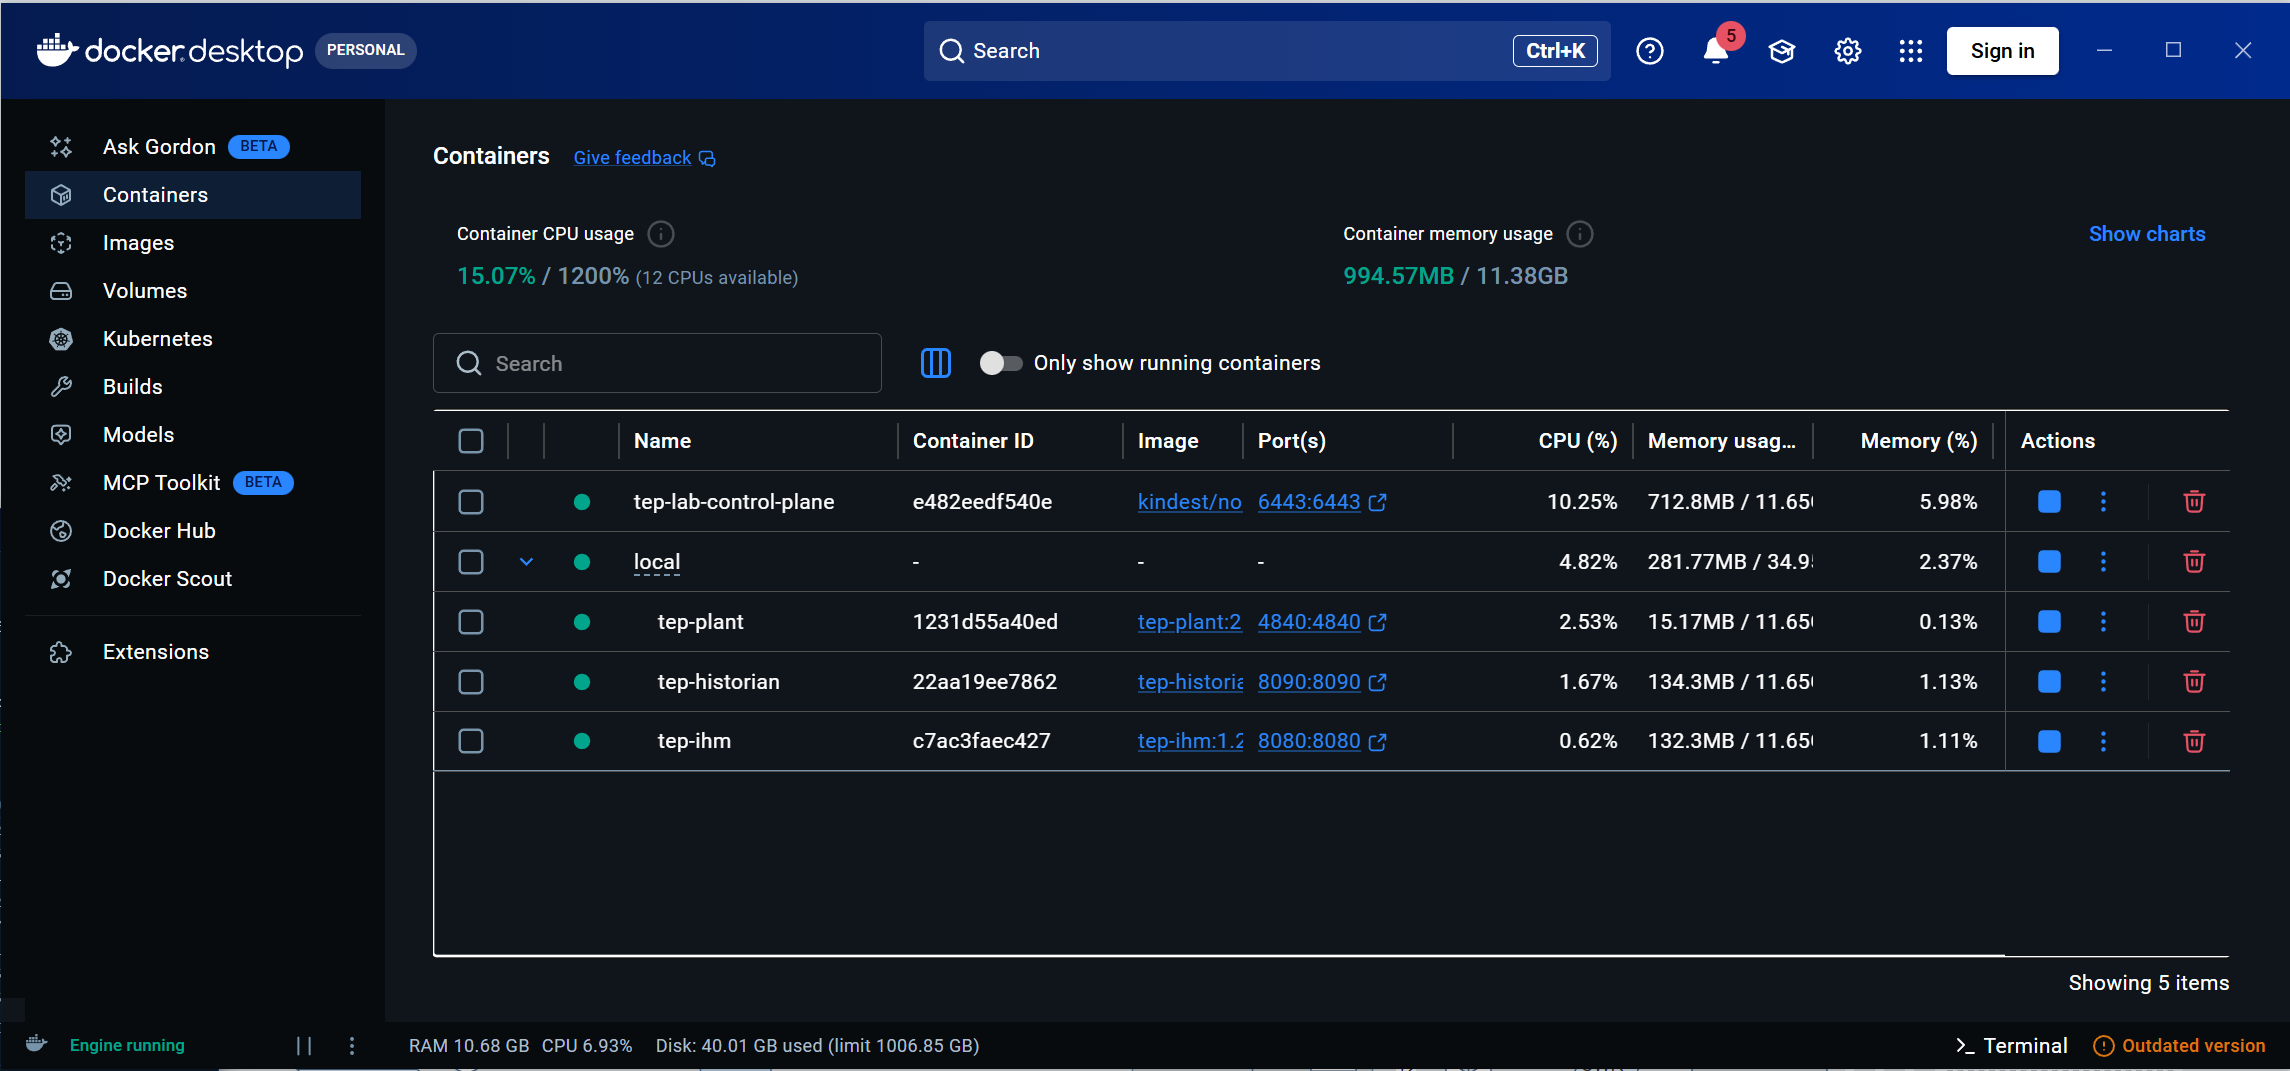
\includegraphics[width=\textwidth]{imagens/containers-rodando-docker.png}
	\fonte{Elaborado pelo autor.}
	\label{fig:docker}
\end{figure}

Com tudo de pé, o acompanhamento é feito com o próprio \texttt{kubectl}. O \texttt{kubectl get plants} mostra o custo e a fase; o \texttt{kubectl describe plant tep} mostra as \textit{conditions}, com as mensagens; o \texttt{kubectl edit operatingpolicy tep-mode1} muda a política com o supervisor rodando, e ele reavalia na hora; e o \texttt{kubectl logs -f deploy/plant-supervisor} mostra uma linha por avaliação. Para destruir o \textit{cluster}, basta o comando \texttt{kind delete cluster -{}-name tep-lab}.

Pela IHM, o mesmo \textit{status} aparece num painel próprio, aberto pelo botão \textit{K8s Supervisor} da barra superior (Figura~\ref{fig:ihm_supervisor}). O painel traz a fase, a política ativa, o custo $J$ com o orçamento e a referência, o número de avaliações ruins seguidas, o instante da última avaliação e o motivo da fase. Abaixo vêm duas tabelas: as metas e os limites da política, com o valor observado de cada sinal, e as malhas de controle, com o índice, o \textit{offset}, o desvio padrão da válvula e o resultado de cada uma. Na captura, a planta estava em operação normal: $J = 166{,}27$~\$/h, abaixo do orçamento de 170,6~\$/h, com todas as metas, limites e malhas em ordem.

\begin{figure}[htbp]
	\centering
	\caption{O veredito do supervisor visto na IHM: o painel do Kubernetes, com a fase, o custo, as metas e os limites da política e as malhas de controle.}
	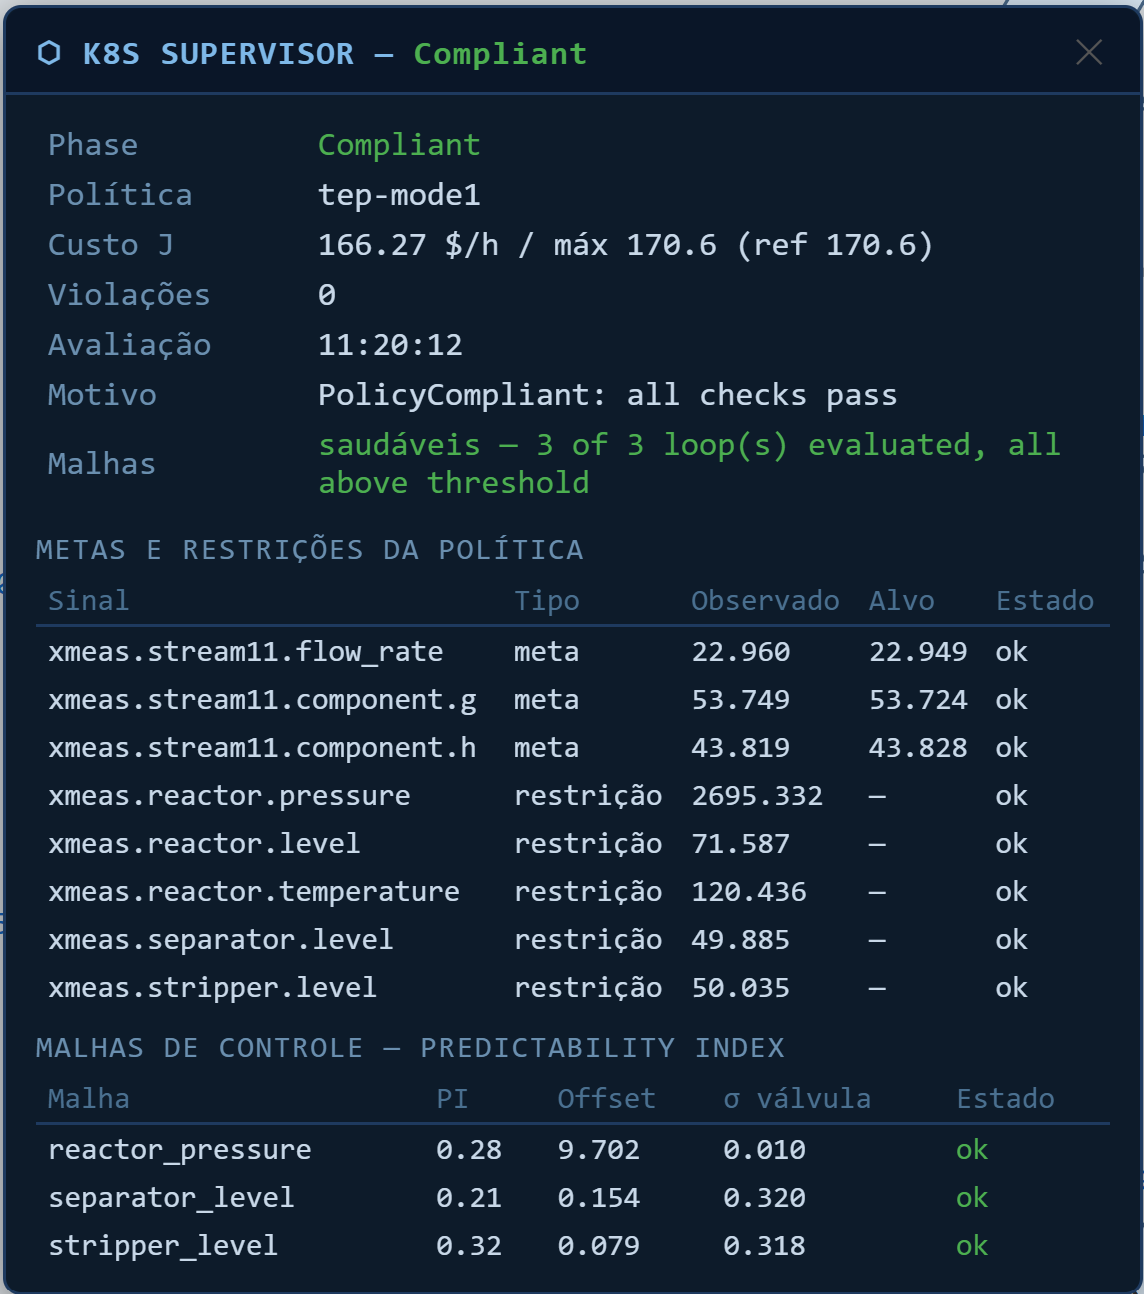
\includegraphics[width=0.5\textwidth]{imagens/foco no painel.png}
	\fonte{Elaborado pelo autor.}
	\label{fig:ihm_supervisor}
\end{figure}

Três \textit{scripts} em Python, na pasta \texttt{scripts/}, gravam os experimentos. O \texttt{record\_run.py} lê a \texttt{Plant} pelo \texttt{kubectl} a cada intervalo e grava num CSV o tempo simulado, o custo, a fase, as \textit{conditions} e o índice de cada malha, porque o \textit{status} só guarda a avaliação mais recente. O \texttt{record\_signals.py} grava, a partir do \textit{historian}, as médias dos sinais que o \textit{status} não traz, como o nível do reator e as posições das válvulas. O \texttt{summarize\_run.py} resume uma gravação, com a distribuição do custo e do índice, e foi usado para escolher os limites da política. Os três usam só a biblioteca padrão do Python.

% -------------------------------------------------------------------------
\section{Experimentos que fizeram a planta funcionar}
\label{sec:experimentos_planta}

Antes de servir aos experimentos com o supervisor, a planta precisou rodar por horas sem sair dos limites. Esta seção resume os experimentos 3 a 11 do registro do projeto, que levaram a planta a esse ponto. Eles foram feitos numa versão anterior do \texttt{tep-plant}, um programa de terminal que gravava os sinais num arquivo CSV, ainda sem comunicação em rede, com os três controladores proporcionais escritos dentro do laço de simulação e o passo de integração de 0,001~h. As conclusões foram levadas para a versão atual. Os experimentos 1 e 2 cuidaram dos gráficos e da partida a frio e não são discutidos aqui.

\subsection{O ponto de partida}
\label{subsec:exp_partida}

Nos primeiros experimentos, a planta partia dos valores iniciais do FORTRAN, com as válvulas de alimentação abrindo aos poucos, e levava tempo para se acomodar. No Experimento~3, a planta rodou 20~h de tempo simulado, sem distúrbio, com os três controladores proporcionais, e o vetor de estados foi salvo num arquivo TOML no fim. O ponto alcançado não é exatamente o do Modo~1 do FORTRAN: a pressão do reator ficou perto de 2680~kPa, contra 2705~kPa no caso base, porque os controladores proporcionais seguram a planta em outro ponto, com um pequeno erro em regime. Mas é um ponto em que essa planta, com esse controle, fica praticamente parada.

No Experimento~4, a planta partiu direto desse arquivo, sem a abertura gradual das válvulas, e rodou 5~h sem nenhuma parada de emergência. A única marca da partida foi um pico nas derivadas no primeiro instante, que sumiu em menos de 0,01~h simulada. A partir daí, todos os experimentos passaram a partir desse arquivo. O \texttt{application.toml} da versão atual é esse mesmo arquivo (Código~\ref{cod:toml}), e é por isso que a planta já começa operando, sem transiente de partida.

\noindent\begin{minipage}{\linewidth}
\begin{lstlisting}[language=toml, caption={Trechos do \texttt{application.toml}, com o estado salvo no Experimento~3}, label={cod:toml}]
[meta]
mode = 1
description = "TEP snapshot at t = 20.0000 h"
source = "auto-snapshot from simulation"

[state.reactor_vapor]
A = 10.679592788064898
B = 4.666690921054032
# ... C a H

[state.reactor]
energy = 2.6983891373872186

# ... separador, stripper, compressor e água de resfriamento

[state.valves]
d_feed                    = 63.05263038999999
# ... as outras 11 válvulas
\end{lstlisting}
\fonte{Elaborado pelo autor. \texttt{tep-plant}, arquivo \texttt{application.toml} (trechos).}
\end{minipage}

Esse ponto foi obtido por simulação, e não por otimização. Hoje, o \texttt{tep-optimizer}, o trabalho paralelo citado na Seção~\ref{subsec:otimizacao}, calcula pontos de equilíbrio e o ótimo econômico do Modo~1 diretamente, chamando a planta como uma função. Ele chegou ao ótimo publicado por \citeonline{Ricker1995}, de 114,3~\$/h, mas está fora do escopo deste trabalho, e a planta não parte dos pontos que ele calcula.

\subsection{A oscilação do reciclo e o acúmulo de gás}
\label{subsec:exp_acumulo}

Partindo do arquivo, a vazão de reciclo (XMEAS 5) oscilava cerca de $\pm 0{,}5$~kscmh o tempo todo, enquanto os outros sinais ficavam estáveis. No Experimento~5, o passo de integração foi reduzido dez vezes, e a oscilação não mudou, o que descartou um efeito numérico. No Experimento~6, os estados internos do reator e do compressor passaram a ser gravados, e eles eram lisos: a oscilação estava só na medição, que no modelo tem ruído. O mesmo experimento mostrou outra coisa, mais importante: os inventários de gás do reator e do compressor cresciam devagar, cerca de 0,4 a 0,5~kmol/h cada.

No Experimento~7, o \textit{setpoint} de pressão foi mudado para o valor em que a planta de fato operava, para abrir um pouco mais a purga. O acúmulo só mudou de lugar, do compressor para o reator. No Experimento~8, os oito componentes do inventário do reator foram olhados um a um, e todos cresciam na mesma proporção, com a composição constante. Isso não era o acúmulo de um produto ou de um inerte, mas um desbalanço global, com um pouco mais de gás entrando do que saindo. A hipótese seguinte foi a de que faltava uma quarta malha, que segurasse o inventário total. No Experimento~9, uma malha do nível do reator para a alimentação de A foi acrescentada, e o acúmulo ficou cerca de seis vezes pior. A pressão subia, o equilíbrio líquido-vapor empurrava material para o líquido, e o nível subia como efeito, e não como causa: a malha agia sobre o sintoma. Ela foi retirada e não existe na versão atual.

Com isso, a busca por um estado estacionário perfeito foi encerrada. O acúmulo era de cerca de 1~kmol/h, ou 0,15~\% do inventário de gás por hora, e diminuía com o tempo, pouco para rodadas de 10 a 20~h. O TEP foi proposto para estudar a rejeição de distúrbios, e esse passou a ser o foco.

\subsection{A linha de base e os controladores separados da planta}
\label{subsec:exp_base}

O Experimento~10 é a linha de base: 20~h sem distúrbio, partindo do arquivo, com os três controladores (Figura~\ref{fig:exp10}). A planta não se aproximou de nenhum limite de parada. A pressão foi de cerca de 2680 para 2700~kPa, o nível do reator de 69 para 73~\%, e os níveis do separador e do \textit{stripper} ficaram em torno de 50~\%. A figura também mostra o ruído na vazão de reciclo, o inventário de gás do reator subindo devagar e os seus oito componentes crescendo juntos, como visto nos experimentos anteriores. Essa rodada serviu de referência para os experimentos com distúrbios.

\begin{figure}[htbp]
	\centering
	\caption{Linha de base de 20~h sem distúrbio (Experimento~10), na versão anterior da planta: pressões, temperatura, níveis, válvulas, reciclo, purga, derivadas e inventários de gás.}
	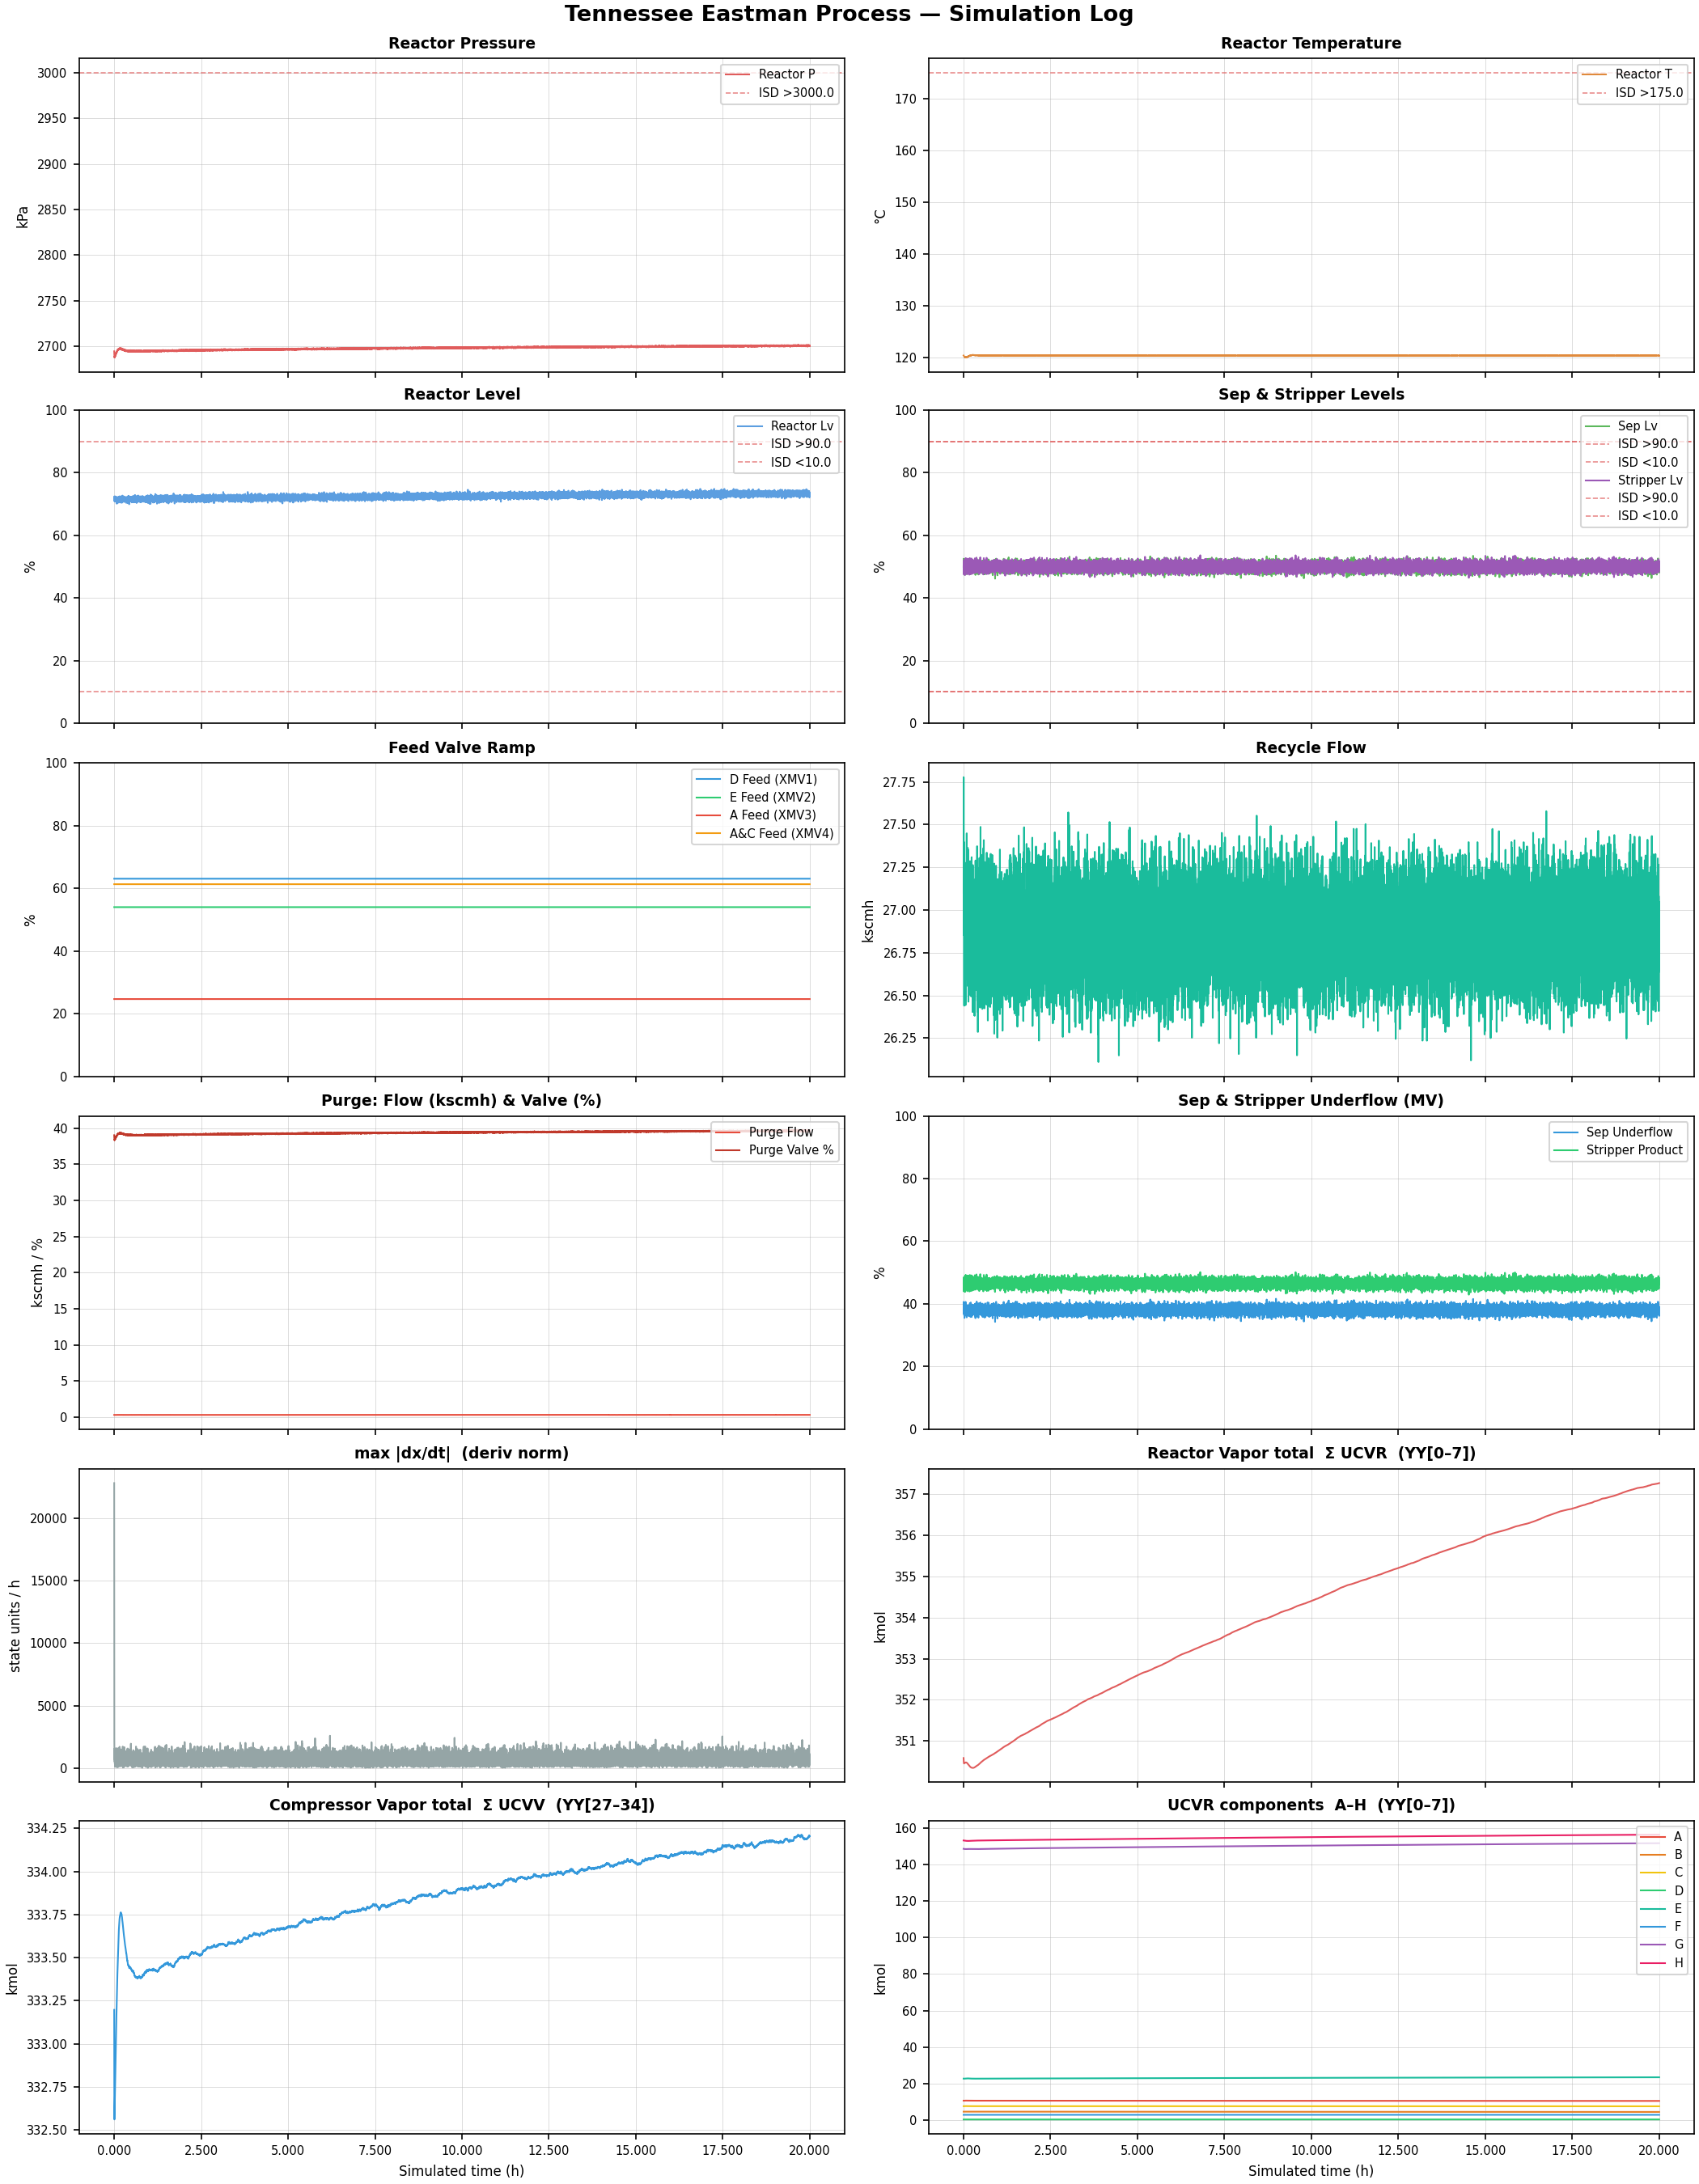
\includegraphics[height=0.78\textheight]{imagens/tep-exp10-linha-de-base.png}
	\fonte{Elaborado pelo autor.}
	\label{fig:exp10}
\end{figure}

No Experimento~11, os controladores, que até então eram três linhas dentro do laço de simulação, foram separados da planta, numa interface própria, com os mesmos ganhos e \textit{setpoints}. A rodada de 20~h gerou um arquivo CSV idêntico, bit a bit, ao da linha de base. A mudança era só de organização, mas foi ela que permitiu, mais tarde, que cada controlador virasse um componente próprio, como os da Seção~\ref{subsec:malhas}.

% -------------------------------------------------------------------------
\section{Considerações finais}
\label{sec:dev_conclusao}

Este capítulo descreveu os componentes do laboratório e o caminho até a planta funcionar. A planta foi reescrita em Rust de um jeito em que quem a escreve trata só do processo e do controle, com três malhas de controle, proporcionais na versão 2.0.0 e PI na 2.1.0-alpha, e cinco dos vinte distúrbios. O \textit{historian} transforma os sinais em estatísticas e no índice das malhas, a IHM mostra a planta e o veredito, e o supervisor no Kubernetes compara a planta com a política de operação declarada nos manifestos, sem agir sobre ela.

Algumas limitações ficaram registradas ao longo do capítulo: os distúrbios aleatórios e as válvulas travadas ainda não existem, a temperatura da água de resfriamento é constante na versão usada, a escala do índice das malhas no código é a oposta da leitura do Capítulo~\ref{cha:referencial}, e os comandos da IHM não chegam à planta. O próximo capítulo mostra os experimentos feitos com o laboratório completo, com os gráficos do custo, das malhas e do veredito do supervisor, com a planta em operação normal e sob distúrbio.
